\begin{figure}[h]
    \centering
    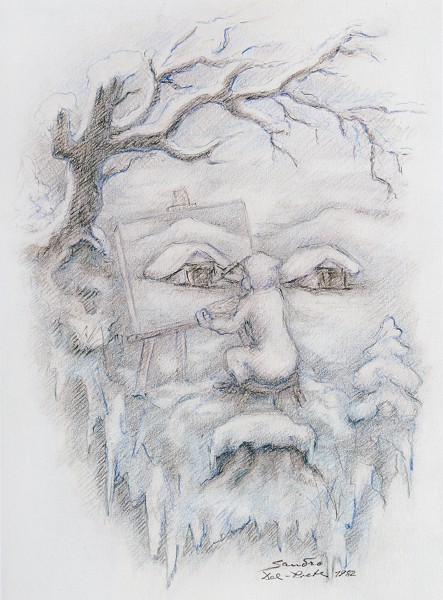
\includegraphics[width=0.8\textwidth]{sdp_mountain_spirit.jpg}
    \caption[Mountain Spirit in Winter by Sandro del Prete]{Mountain Spirit in Winter by \citeay{del_prete_mountain_1982}.}
    \figlbl{sdp_mountain}
\end{figure}

One of the insights from the \emph{Gestalt} psychology \sidecite{ellis_source_1938, kohler_gestalt_1992, wagemans_century_2012, hamlyn_psychology_2017} is that humans are apparently able to recognise the Gestalt of an object within a very short time; The brain can immediately recognize global patterns - arrays of local features that consistently conform to a known large-scale pattern - even if those local features are buried in noise or would, on the basis of local context, be interpreted very differently. Thus, local decisions are made based on plausibility considering overall patterns, while the overall patterns can only be defined based on local features.

For example, when looking at \figref{sdp_mountain}, local and global patterns are not aligned. A painter drawing a picture from a house in a snowy landscape can be observed when looking at local features. However, when looking at the overarching pattern, a man's face is visible.
This example illustrates that, when extracting features from images, it is important to avoid the ``fallacy of early commitment'', as David Marr put it \sidecite{marr_vision_2010}.
Otherwise, when looking at local features only, systems could commit to objects like trees, a painter, an image, a house, and snow. Such systems would not be able to recognise the global pattern as a men's face typically comprises eyes, nose, etc. and not the aforementioned objects.

The theory of natural intelligence \sidecite{von_der_malsburg_theory_2022} and work based on self-organising projection fibres (c.f. \secref{projection_fibres}) considers the principle of preventing early commitment as a core principle for the effectiveness of the human visual system.
Preventing early commitment allows the model to leave multiple options open at the same time: The model does not take decisions at a early stage of the learning process as typical deep learning models do but rather iterate between local and global features, continuously ruling out implausible hypotheses.

The most used architectures for image processing are based on CNNs (c.f. \secref{cnns}). This type of network cannot prevent early commitment by design: The first layers extract local features from images, thereby having access to small patches only. The extracted low-level features are combined into higher-level features in later layers \sidecite{prince_understanding_2023}. Thus, the first layers do not consider global features but steer the decision process during training and inference toward specific directions based on local features. Therefore, CNNs take local decisions without consolidating global information\sidenote{CNNs can be trained to make diverse decisions in high-level layers when appropriate labels are given. However, these decision are still based on already made local decisions and such networks cannot deal with ambiguity since the decision process is not based on a 2-way iteration.}.

Transformer-based \sidecite{dosovitskiy_image_2021} or fully connected \sidecite{tolstikhin_mlp-mixer_2021} vision architectures, on the other hand, might not have this limitation since these architectures can access the entire input.
However, they have a fallacy of early commitment in the sense that they process the input layer-wise. Typically, the input of a vision architecture is specific (e.g. an image) and mapped to more general information (e.g. a class label).
However, general information is not used to confirm or validate specific information and, therefore, high-level decisions can be misled by the wrong and inconsistent early decisions.
Thus, the first layers make decisions on lower-level features and steer the decision process during training and inference towards a specific direction without considering higher-level features, thereby being prone to early commitment as well.

Furthermore, deep learning architectures do not model the concept of uncertainty across different levels, which is a crucial factor to avoid early engagement. In general, these architectures process representations sequentially in a hierarchical manner. At each level, the model generates a representation that is usually a more abstract version of the previous one. Nevertheless, at each level, the network decides on a single representation and thus makes an early commitment. To solve this problem, two measures must be taken: First, it would be beneficial to introduce multiple hypotheses at each layer and restrict the layers to modelling their uncertainties rather than committing to a single hypothesis. Second, the model needs to be able to re-evaluate previously taken decisions, i.e. update local decisions in the light of global decisions.

Thus, deep learning are susceptible to early commitment and cannot effectively capture uncertainty across different levels. Furthermore, they have a lack of dealing with ambiguity and lack invariance to object transformations (c.f. \secref{limitationsDL}).
The inability to deal with ambiguity is related to the fact that deep learning networks do not model uncertainty and usually provide a single prediction. In addition, object transformations are not handled independently of the object. Therefore, deep networks require multiple views of each object to interpolate the underlying data\sidenote{On of the main reasons why data augmentation is needed for the training of deep networks.}.
To mitigate these disadvantages, a biologically inspired vision framework is proposed. 
The framework is on the verge between the two fields of neuroscience and deep learning.
Both fields use similar vocabulary, but sometimes refer to different principles. 
Therefore, some general principles from neuroscience and a unified vocabular are introduced first.
The subsequent sections provide an overview of the framework, highlight its advantages and explain the inspiration for its design. Next, the components of the framework are explained in more detail.



\section{Neuroscientific Inspiration and Vocabulary}
Readers of this work are expected to be primarily people with a background in computer science or neuroinformatics. However, in order to understand the fundamental principles underlying the proposed framework, understanding of neuroscience findings and vocabulary is required. Therefore, this section explains the neuroscientific inspirations and key terms related to this work.

The neuroscience concepts presented in this thesis are simplified to make the proposed framework comprehensible to readers from various fields. Experts from the field of neuroscience may find this section superfluous and may skip it.

\begin{figure}[h]
    \centering
    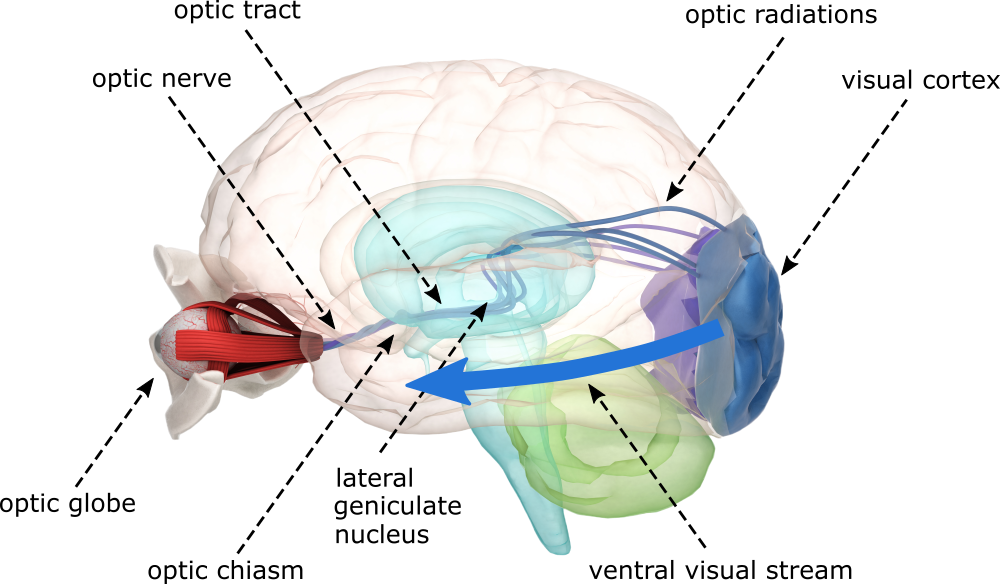
\includegraphics[width=0.99\textwidth]{Visual-System}
    \caption[Visualisation of the human's visual system]{Visualisation of the human's visual system. The image is from \citeay{fasoli_human_2023}.}
    \figlbl{visual_system}
\end{figure}

\paragraph{The Brain's Visual System.} The visual system of humans is visualised in \figref{visual_system}. The eyes function as sensors that capture light waves and translate them into a electrical pulses. This signal travels through the human brain to the primary visual cortex, located at the back of the head.
Cells within the visual cortex fire a spikes when specific visual stimuli appears within their receptive fields. Thus, these cells can be considered filters that are excited if a specific pattern is detected in the input data. The brain implements this behaviour by utilising lateral connections and net fragments. These fundamental functions of the brain are introduced in the following.

Simply put, the visual cortex detects patterns in visual data. However, it does not draw conclusions from this data but forwards it as an information stream to other areas in the brain. In this thesis, especially the ventral visual stream is of importance. This stream forwards the detected patterns to the temporal cortex, a region of the brain located behind the ears.
According to the two-stream hypothesis \sidecite{goodale_separate_1992}, the temporal cortex is responsible for visual object identification and recognition. There exists a second stream, called the dorsal stream, that forwards the same data to the parietal cortex, a region on top of the head that predicts the object's spatial location relative to the viewer. However, this stream is of less importance in this thesis. The biological mechanism for object identification and recognition is based on projection fibres. These fibres are introduced at the end of this section.


\begin{figure}[h]
    \centering
    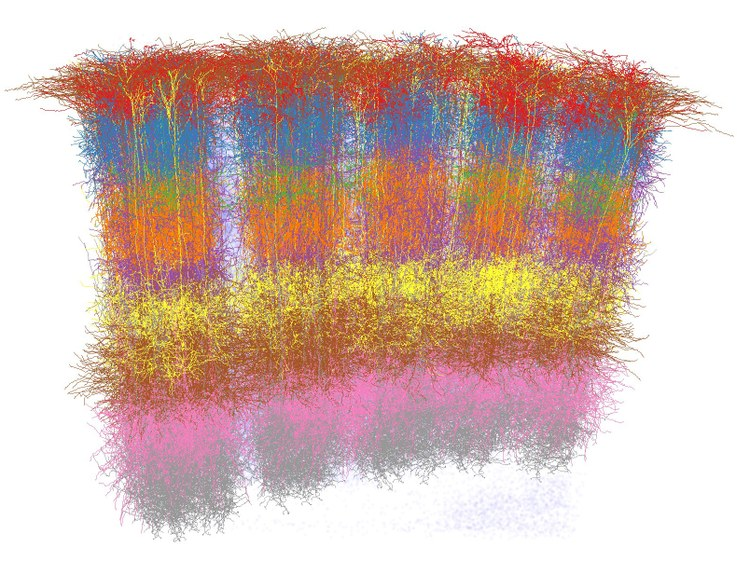
\includegraphics[width=0.99\textwidth]{cortical_columns}
    \caption[3D reconstruction of five neighbouring cortical columns]{3D reconstruction of five neighboring cortical columns of a rat. The image is from \citeay{oberlaender_beyond_2012}.}
    \figlbl{cortical_columns}
\end{figure}

\paragraph{Lateral Connections and Lateral Support.} Typical deep learning architectures process data sequentially, propagating it from one layer to the next. 
This process is inspired  by the layer-wise forward pass observed in the human brain.
However, a closer look at the human brain reveals that there are also connections between neurons within the same layer \sidecite{gilbert_lateral_1990}.
\figref{cortical_columns} visualises a 3D reconstruction of five cortical columns \sidecite{mountcastle_columnar_1997}. Cortical columns are a cylindrical structures of neurons, found in the cerebral cortex\sidenote{The cerebral cortex is well developed in humans and is often associated with intelligence \cite{narr_relationships_2007}.}. 
The different layers within these cortical columns are visualised in \figref{cortical_columns} with different colours.

Unlike typical deep learning networks where information flows sequentially from one layer to the next, a single layer within a cortical column does not solely process information in a sequential manner. The 3D reconstruction in \figref{cortical_columns} also shows connections between neurons in the same layer.
These intra-layer connections are called \emph{lateral connections} and are visualised in a simplified manner in \figref{lateral_connections} for a single neuron.
This neuron not only has connections to neurons in the preceding and subsequent layers, but also has (lateral) connections within its own layer (marked in red).

\begin{figure}[h]
    \centering
    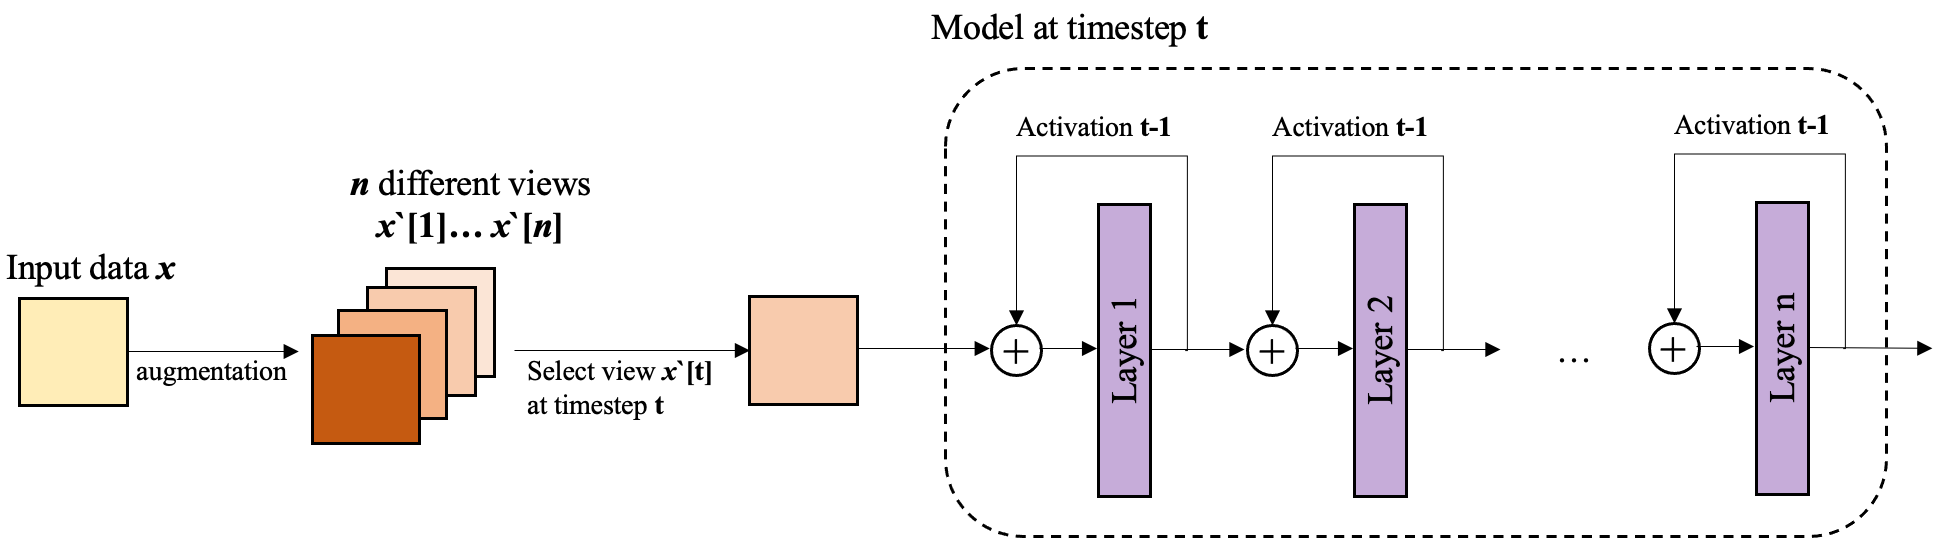
\includegraphics[width=0.99\textwidth]{lateral_connections}
    \caption[Lateral connections of a cell]{Visualisation of the connections of a single cell. The cell is connected to the previous layer (orange), the subsequent layer (green), and to neurons within the same layer (lateral connections, red).}
    \figlbl{lateral_connections}
\end{figure}

According to \sideciteay{von_der_malsburg_theory_2022}, these lateral connection are used for \emph{lateral support}. Lateral support means that neurons from the same layer support another neuron:
Neurons from the preceding layer can activate the red cell in \figref{lateral_connections} through the orange connections.
However, inhibitory signals can suppress the activity of the red neuron before it has a chance to fire a spike to the subsequent layer via the green connections. The neuron can only transmit a spike to the subsequent layers if it ``survives'' the inhibition phase. Remaining active is only possible if the neuron receives sufficient lateral support from neurons within the same layer that are connected with lateral connections.
If the preceding layer activates several neurons within the same layer as the red neuron and these activated neurons exhibit lateral connections, they can send spikes to each other, thereby providing mutual support. This allows them to maintain their action potential and remain active during the inhibition phase.

\paragraph{Net Fragments.} Lateral connections grow between cells that are often active together.
Since similar patterns activate the same neurons, the connection between neurons that represent the same pattern is strengthened. 
Consequently, the strength of lateral connections increases between neurons representing frequently occurring activation patterns, resulting in increased lateral support between groups of neurons. Such groups that represent frequently occurring patterns and have strong lateral connections are called \emph{net fragments}.
All neurons within a net fragment support each other so that they can remain active during an inhibition phase. 
Thus, a layer with multiple net fragments can be considered a filter: While the previous layer might activate numerous cells, only the cells with sufficient lateral support remain active.

\begin{figure}[h]
    \centering
    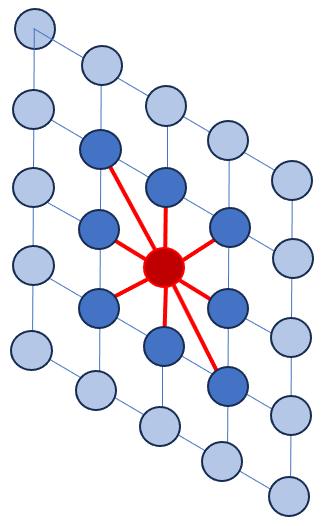
\includegraphics[width=0.5\textwidth]{local_neighbourhood2}
    \caption[Lateral connections limited to a local neighbourhood]{The lateral connections limited to a local neighbourhood.}
    \figlbl{local_neighbourhood2}
\end{figure}
\paragraph{Local Neighbourhood.} Net fragments represent pattern found in the source data. Such patterns can be distinguished between  local patterns, which are spatially limited to a local area, and global patterns, which extend over larger regions of the image and might encompass the entire image.
The number of possible patterns increases exponentially with the size of the considered patterns. Thus, local patterns occur more frequently, while global patterns are rather unique (i.e. an image is only once in the dataset).
In order to learn frequently occurring patterns, the range of the lateral connections must be limited to a \emph{local neighbourhood}, similar to convolutional filters (c.f. \secref{}).
Otherwise, each cell would be directly connected to each other cell in the layer and the lateral connections would capture global patterns.
By limiting the lateral support to local neighborhoods, cells are only influenced by nearby cells and local patterns. This allows the layer to become translation invariant and robust to global transformations. 
\figref{local_neighbourhood2} illustrates such limited lateral connections: The lateral connections from the red cell do not encompass the entire image, but are only connected to cells that are in close proximity.

\paragraph{Overlay Net Fragments.} Net fragments are formed at any point in the network. This results in an overlay of net fragments, which can be interpreted as a larger net fragment, i.e. a multitude of cells supporting each other.
The size of a net fragment cannot be defined; the smallest possible net fragment is a single cell with its lateral connections to the neighbouring cells while the largest possible net fragment can span all active cells that are laterally connected within a layer. 

A single cell is supported by its neighbouring cells which are supported by other cells as well. Therefore, the support reaches much further than only the local neighbourhood.
As the processing progresses, increasing inhibition causes cells without sufficient support to be turned off. Turning off one cell can trigger a chain reaction of further turn-offs. Therefore, lateral support occurs not only between individual cells but also between overlapping net fragments.

\paragraph{Brain's Solution to Prevent Early Commitment.}
Es described in the previous section, deep learning models are prone to early commitment.
The brain's solution to prevent early commitment are net fragments.
A single layer with lateral connections that forms net fragments can represent local and global features at the same time\sidenote{This way of thinking about features can be hard to comprehend, especially for computer scientists familiar with deep learning (including the author of this thesis).}.
Each set of neuron that is active and laterally connected can be considered a net fragment. Net fragments with a small number of cells depict local features, while fragments containing a large number of features represent global features.

A system that avoids the fallacy of early commitment should fulfil the conundrum that local decisions are taken on the basis of plausibility in the light of high-level patterns, while high-level patterns can only be defined on the basis of low-level features.
The most fundamental local decision is to decide if a single cell should be active. Since a single cell receives support from all cells in the largest possible net fragment,
the human brains makes this decision based on a high-level pattern (i.e. based on the activity of all directly or indirectly laterally connected cells), thereby fulfilling the first principle. The high-level pattern used to make this decision is defined by the sum of individual cells. Hence, the second principle is also fulfilled, as the cells are low-level features that define the high-level pattern.

\paragraph{Local Learning Principle.} In the brain, consistency is evaluated at the level of individual synapses. Each synapse is established if the firing of its source neuron and its target neuron are consistent with each other, allowing the source neuron to predict the activity of the target neuron. This process is crucial for the establishment of net structures, where each neuron within a net fragment can predict with high probability the firing of other neurons.
This local learning is a key difference between natural (animal or human) learning and the frequently used backpropagation of error. With backpropagation, consistency is optimized at a single point, specifically between the system's output and a teacher signal. All synapses, including thos that are distantly connected (the ``deep'' connections) are guided by the consistency of this this single point.

\paragraph{Projection Fibres, Maplets, and Control Units.} As described at the beginning of this chapter, the visual cortex extracts pattern from visual information. This process is is implemented with the aforementioned building blocks such as lateral connections and net fragments. In theory, this is sufficient to implement the principles from the Gestalt psychology. However, it is not sufficient for efficient visual object detection.

In the human brain, object detection takes place in the temporal cortex.
However, the visual and temporal cortex are spatially distant from each other.
The brain's solution to transmit information over such long distances are \emph{projection fibres} \sidecite{greig_molecular_2013}.
Projection fibres are links between net fragments in the visual cortex and object prototypes in the temporal cortex, also known as \emph{maplets} \sidecite{zhu_maplets_2004}.

Object prototypes in the temporal cortex are net fragments similar to the ones found in the visual cortex. However, the fragments in the visual cortex are an overlay of multiple fragments that were captured by the eyes.
This overlay of fragments are a description of a captured visual scene, whereby it is unclear which sub fragments represent objects and how they are related to each other.
The fragments in the temporal cortex, on the other hand, depict exactly one single object, whereby these objects are position and transformation invariant.

Projection fibers map net fragments from the visual cortex to object prototypes in the temporal cortex with one-to-one connections \sidecite{anderson_shifter_1987}, where pairs of neurons connected in the visual cortex project to pairs of neurons connected in the temporal cortex. The projection fibers have some flexibility, allowing for local distortions and enabling transformation- and position-invariant mapping. This mapping allows the recognition of one or more objects in a scene and their relationships to each other, facilitating object recognition and scene interpretation. Furthermore, the mapping is independent of objects and enables object recognition even when the object is distorted in a way not present in the data.

Each existing net fragment is mapped to one or multiple object prototypes. Consequently, there is a multitude of projection fibres, but only a fraction of them are active at any given time. \emph{Control units} decide which projection fibres are activated and thus initiate the mapping visual and temporal cortex. Control units trigger a mapping when a net fragment in the visual cortex matches well another fragment in the temporal cortex, i.e. when these two fragments have a high correlation. However, they only remain active if numerous other projection fibres confirm the decision and map their respective fragments in the visual cortex to the same object prototype. By doing so, the human brain generates numerous hypotheses about observations, but inhibitory signals quickly deactivate most projections, leaving only the plausible ones active.

Projection fibres thus provide generalisation, i.e. different, transformed, versions of an object can be mapped to each other. This explains the ability of humans to see a new object once and immediately recognize it in transformed version.

\paragraph{Emergence.} One question that constantly puzzles the field of AI is whether a system exhibits an emergence of intelligence.
This question also has many philosophical aspects and cannot be answered conclusively within the scope of this thesis.
Based on the authors intuition, and without any formal proof, the proposed framework could exhibit emergence.
In the context of visual processing, emergence refers to the ability of a system being able to interpret scenes by putting high-level decisions, such as objects, in relation to each other. This ``putting in relation'' is possible with the help of a coherent net that interprets the whole scene, relative to which isolated part-interpretations lose out by lack of support. Such a coherent net could be implemented with net fragments and projection fibres, where projection fibres map scenes to interpretation and the internal support algorithm ensures that the network reaches a consistency between all elements, i.e. object's within a scene, their relation, and a possible interpretation.
However, this is only possible of consistency is achieved at every single point in the network.
This concept of creating consistency could be the missing part to achieve emergence.








\section{3-Staged Model}

TODO: DELETE THIS IMAGE? -> See comment Thilo

\begin{figure}[h]
    \centering
    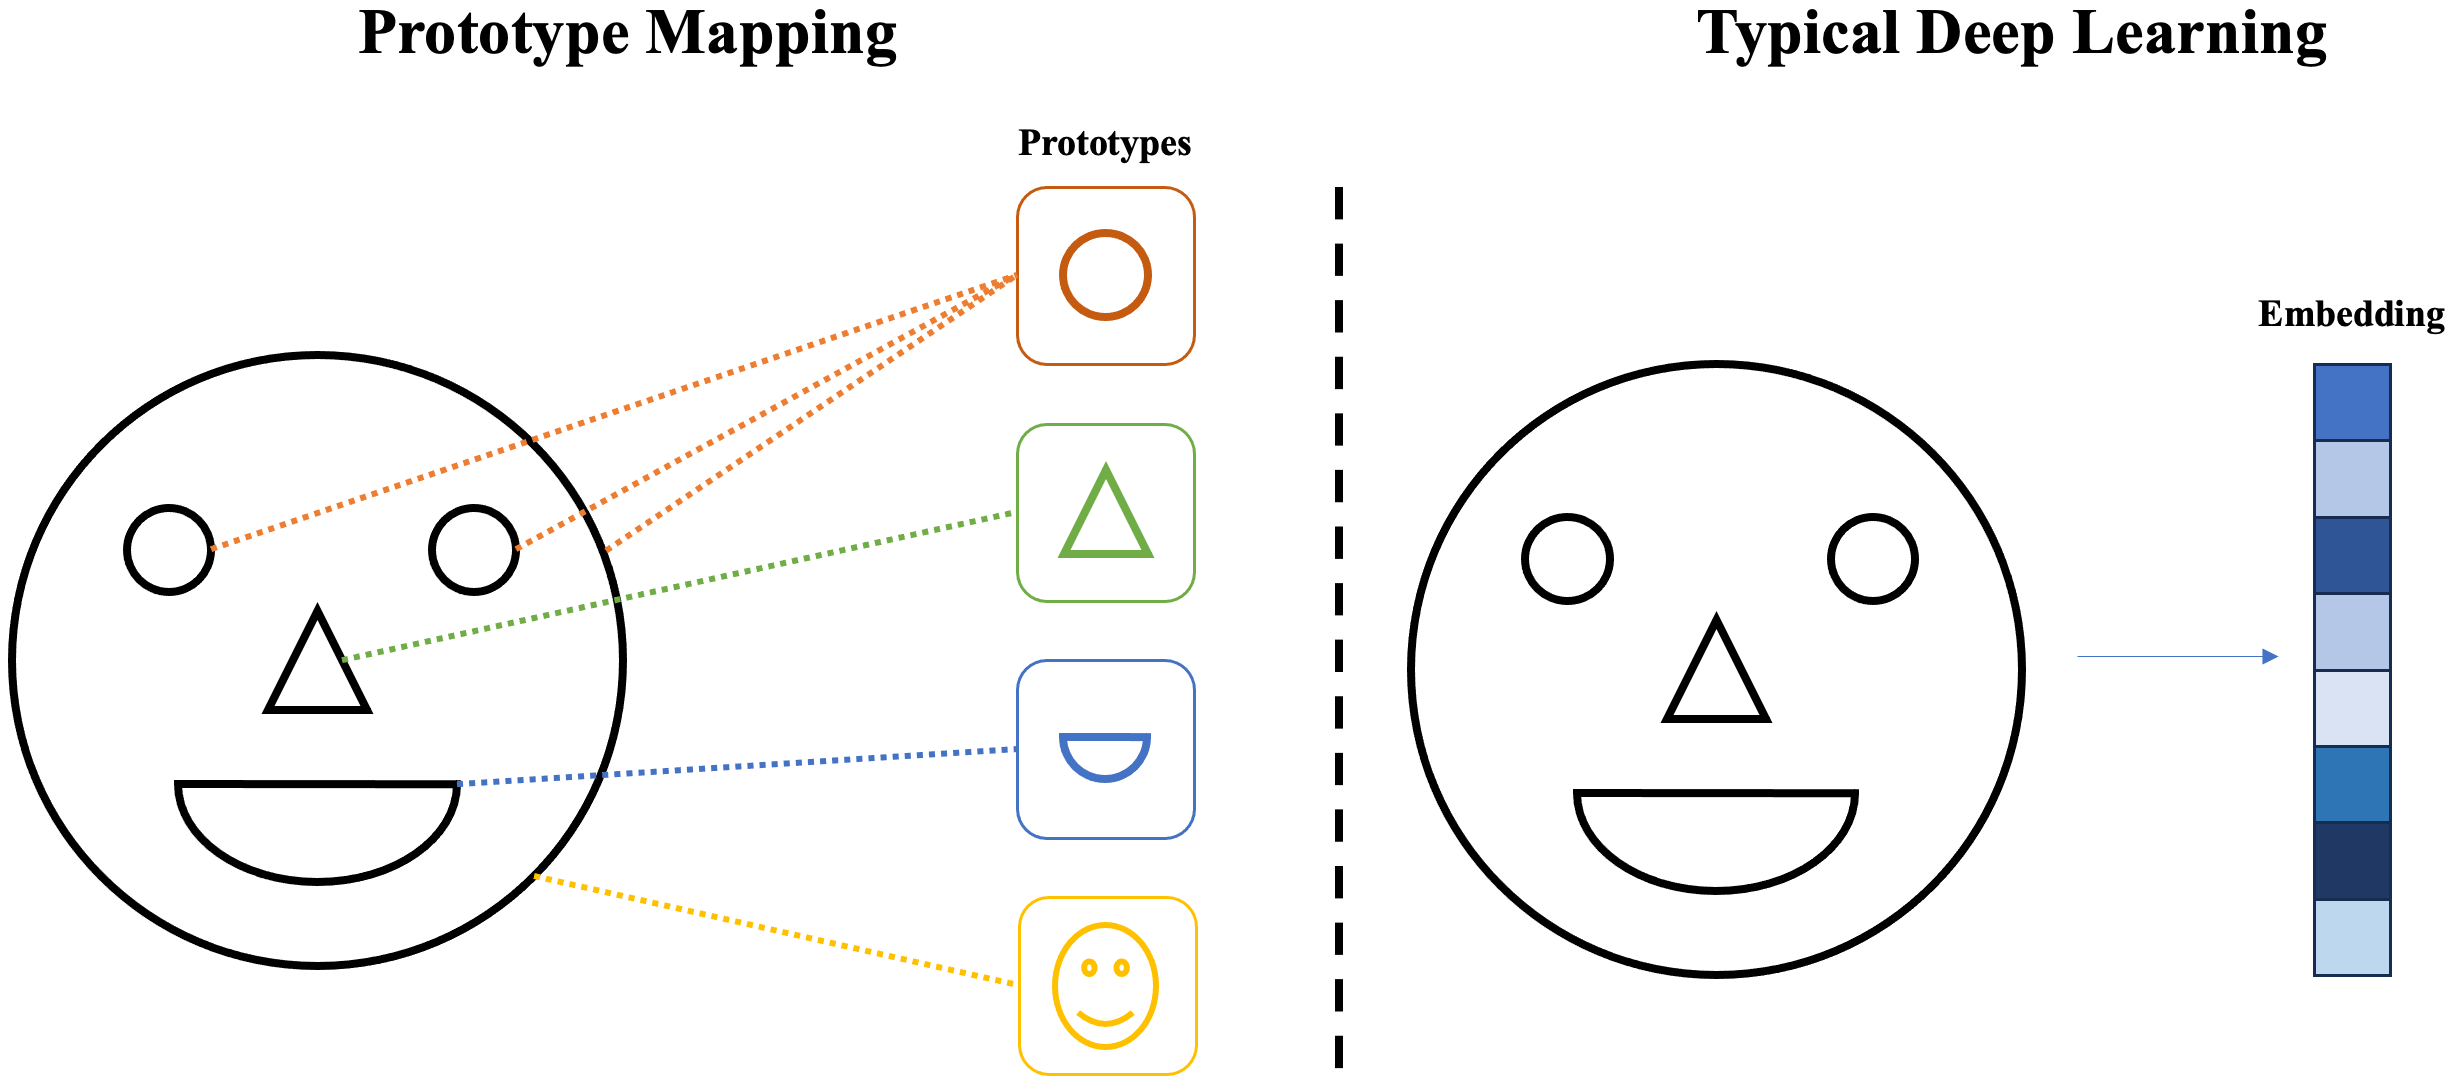
\includegraphics[width=0.99\textwidth]{prototype_mapping}
    \caption[Mapping from an image to prototypes]{Mapping from an image to prototypes and vice versa in contrast to deep learning models.}
    \figlbl{prototype_mapping}
\end{figure}








The only solution is to iterate between local and global features, refining them in a coarse to fine manner \sidecite{wiskott_face_1996, wolfrum_recurrent_2008}. This process requires a two-way mapping from local features to prototypes and vice versa, as visualized in \figref{prototype_mapping}.
Thus, the system should be able to map parts of an image to meaningful prototypes, as shown on the left, and not just compress the entire image to an embedding representation as typically done in deep learning applications \sidecite{prince_understanding_2023}.
Such systems have been explored in the theory of self-organising projection fibres (c.f. \secref{projection_fibres}), however, did not yet scale to natural images except for human faces \cite{wolfrum_recurrent_2008}.

This section describes a system that might scale to natural images.
It is based on three main components: A sensory stage \emph{S0} that extracts features from the image, a stage \emph{S1} building local features, and a stage \emph{S2} mapping these local features to object prototypes by utilising projection fibres.
In the context of biology, the sensory stage \emph{S0} could stand for the eyes translating visual information into neuronal activity, \emph{S1} could stand for the primary visual cortex \sidecite{tong_primary_2003, grill-spector_human_2004}, and \emph{S2} for an area in the temporal cortex \sidecite{miyashita_inferior_1993, conway_organization_2018}.
These three building blocks are described in the following.











\subsection{Building Blocks}
\begin{figure}[h]
    \centering
    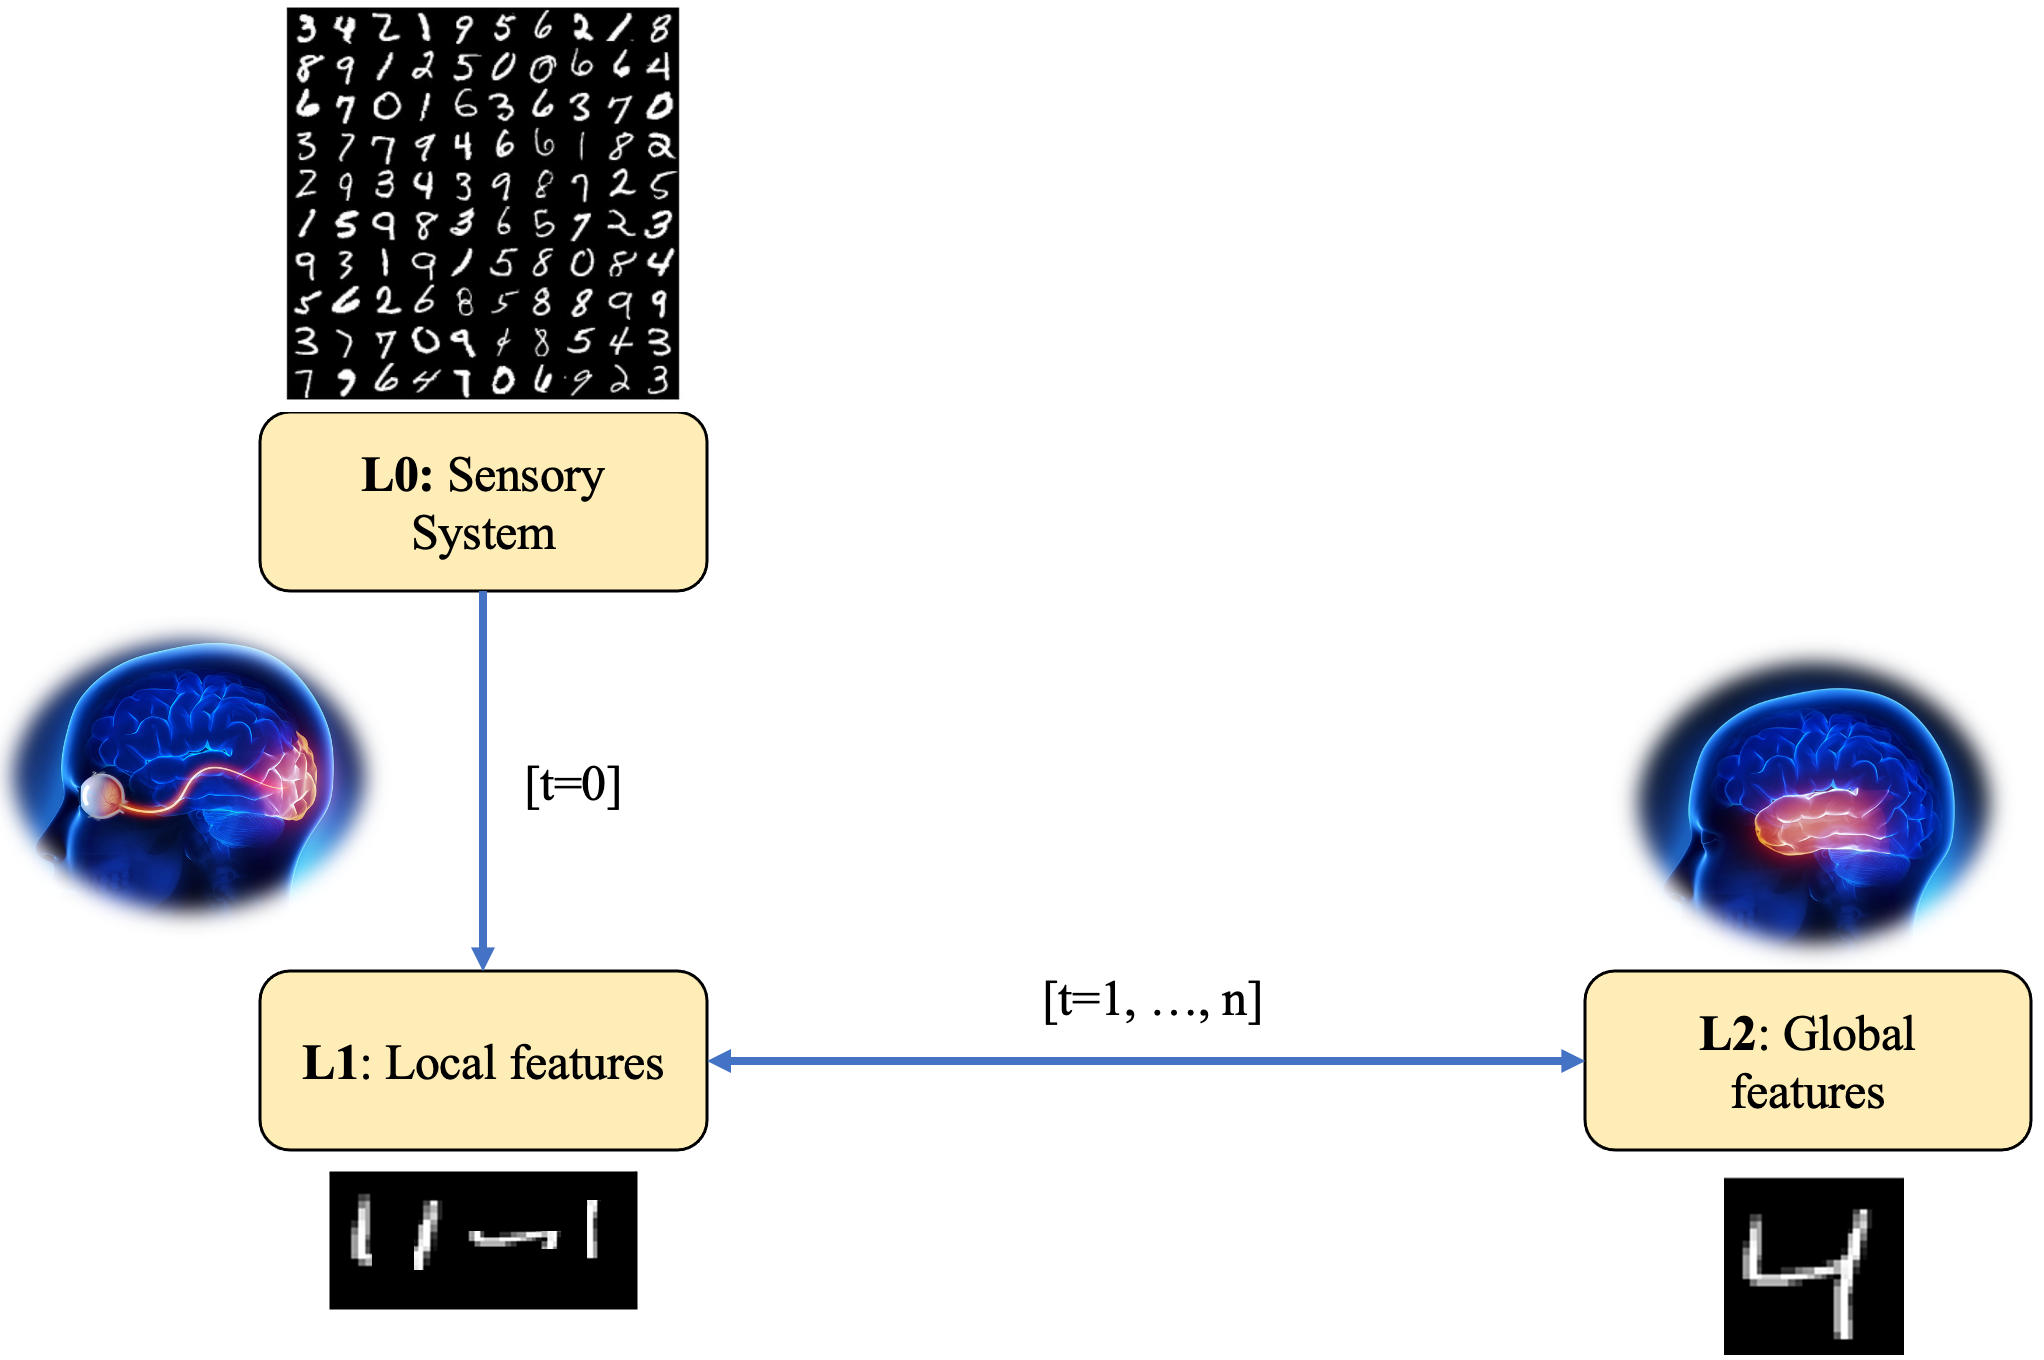
\includegraphics[width=0.99\textwidth]{system ovierview}
    \caption[Overview of the framework]{Overview of the framework. \emph{S0} extracts features from the image at timestep $t=0$, \emph{S1} builds local features, and \emph{S2} maps them to global features. The network refines the features over multiple timesteps by iterating between local and global features.}
    \figlbl{system_overview}
\end{figure}

\figref{system_overview} provides an overview of the building blocks of the proposed framework. The Sensors system \emph{S0} extracts features from an input image. These features are refined over multiple timesteps by iterating between local and global feature processing, thereby preventing the system from early commitment.

\paragraph{Sensors System \emph{S0}.} The sensory stage \emph{S0} extracts features from the image that are forwarded to \emph{S1}.
A typical input to the sensory stage is an image having one (grayscale) or three (RGB) colour channels. Therefore, such an image can be interpreted as having one or three features at every spatial location.
The sensory system extracts multiple higher-level features by considering a spatially local neighbourhood. Thus, the number of features is increased by the sensory system.
A sensory system can be, for example, a set of hand-crafted filters or Gabor filters that are shifted across the image, or the first layer of a pre-trained CNN model.

\paragraph{Local Features Stage \emph{S1}.} The local feature stage is a single layer with short-ranging lateral connections \sidecite{gilbert_lateral_1990}, allowing neurons in a spatially narrow neighbourhood to support each other. Input from the sensory system activates some feature neurons in \emph{S1}. However, their continued firing relies on receiving support from a sufficient number of other activated neurons that are laterally connected to them. Initially activated neurons that do not receive enough lateral support deactivate after a short period due to inhibition \sidecite{coombs_specific_1955}.

The lateral connections are learned through self-organisation. Patterns occurring repeatedly in the training data will constantly activate the same cells simultaneously. Using Hebbian learning strengthens the connection between these cells, and the pattern is ``stored'' in a net fragment. The inhibition strength increases during training so that only frequently occurring patterns can lead to constant cell activation.

Consequently, many neurons might be activated by the sensory stage, but only the ones supporting each other remain active.
Therefore, it is essential to view the process from the perspective that neurons that remain active are integral parts of consistent net fragments, and only the support from neurons within the same net fragments enables them to persist.
The connections present in \emph{S1} possess the capacity to represent an extensive array of consistent connectivity patterns. Each neuron within \emph{S1} exhibits multiple excitatory incoming and outgoing connections, allowing it to be involved in slight variations and deformations of a specific pattern and completely distinct global patterns. However, due to the limited range of lateral connections, coherence is maintained only within that particular range.

\paragraph{Global Features Stage \emph{S2}.} Long-range connections are essential to represent larger-scale structures like an object. In \emph{S2}, large patterns, typically representing objects, are stored. 
It has a smaller coverage area, focusing specifically on object-centred representations rather than encompassing the entire visual field.
The patterns in \emph{S2} remain invariant to translation, scale, and orientation, enabling the incorporation of broader spatial relationships.

In the object recognition process, corresponding net fragments in \emph{S1} are mapped to object prototypes in \emph{S2} through active projection fibres. Here, ``corresponding'' refers to neurons relating to the same point on the object's surface.
The projection fibres between \emph{S1} and \emph{S2} are composed of ``maplets''. A maplet comprises a collection of fibres that establish one-to-one connections between all neurons in a small patch of \emph{S1} and all neurons in a small patch of \emph{S2} in a topological manner. This topological connection links neighbouring neurons in \emph{S1} to neighbouring neurons in \emph{S2}. Both \emph{S1} and \emph{S2} are divided into overlapping patches, and for each pair of patches — one in \emph{S1} and one in \emph{S2} — a corresponding maplet exists.

Control units are used to activate projection fibres.
Control units initiate activation when they observe a high pattern correlation between the fibres reaching \emph{S1} and \emph{S2}. They inhibit competing units and stabilise the network in \emph{S2} using the activated fibres. Consequently, the activated projection achieves a homeomorphism, where neurons of a particular feature type in \emph{S1} are connected to neurons of the same type in \emph{S2}.

\paragraph{Bernoulli Neuron.} The aforementioned components are implemented using on a novel type of neuron, called the Bernoulli neuron (c.f. \secref{bernoulli_neuron}). This neuron interprets the incoming activity as an activation probability and samples a binary signal from a Bernoulli distribution based this probability. Utilising Bernoulli neurons lead to sparse and distributed binary network activities, which possess properties that enhance robustness to noise within a network \sidecite{ahmad_properties_2015}.

Furthermore,  Bernoulli neurons allow to model net fragments with lateral support. Preliminary experiments have indicated that using non-binary artificial neurons is not well suited for learning net fragments. For instance, dealing with very weak or strong positive activations poses challenges when employing Hebbian updates. In contrast, the Bernoulli neuron tends to convert negative negative or very weak activations to $0$, while strong activations tend to become $1$. This behavior prevents the establishment of connections between weakly activated neurons. Furthermore, sampling from a Bernoulli distribution introduces a small amount of noise to the network, encouraging parallel paths and increasing robustness (c.f. \secref{bernoulli_neuron}).



\subsection{Relation to Theory of Natural Intelligence}
The mapping between input data and stored object prototypes is closely related to the human brain's functionality and in line with findings from neuroscience \cite{kandel_principles_2013, olshausen_emergence_1996, vogels_inhibitory_2011, payeur_burst-dependent_2021} and psychology \cite{ellis_source_1938, kohler_gestalt_1992, wagemans_century_2012, hamlyn_psychology_2017}.

The theory of natural intelligence by \sideciteay{von_der_malsburg_theory_2022} describes how the brain develops an overlay of net fragments (c.f. \secref{natural_intelligence}). These attractor networks consist of neurons supporting each other to remain active.
This behaviour is implemented in the local feature stage \emph{S1}: The sensory signal from \emph{S1} activates many neurons from which only the ones receiving enough lateral support remain active. The neurons that support each other thus build a net fragment.

The theory also describes that an object is represented by multiple net fragments, whereby each net fragment represents a part of the surface of that object.
As described above, net fragments are built in \emph{S1} but are restricted to a spatially local neighbourhood. Projection fibres map these net fragments to object prototypes in \emph{S2}. Thus, an overlay of attractor networks represents an object, as suggested in the theory of natural intelligence.

Furthermore, it is postulated in the theory that self-organisation is the key algorithm to form such fragments and the learning mechanism loops between activity and connectivity for a short time until an attractor state is reached.
In the context of this work, self-organisation is used to organise the lateral connection in \emph{S1}. In fact, local Hebbian learning is applied to learn the support strength between neurons, allowing the network to turn off neurons that are not part of the dominating net fragments.
Furthermore, looping between activity and connectivity is implemented with projection fibres. 
Each prototype in \emph{S2} is considered a hypothesis of what object is present in the input. A net fragment can be mapped to multiple prototypes, and each active net fragment supports specific hypotheses in \emph{S2}. The hypotheses act back on \emph{S1} and, in turn, support local net fragments. Thus, the activity part is realised by \emph{S1} when supporting or turning off cells and the connectivity part is realised by projection fibres mapping the net fragments to \emph{S2}, thereby providing feedback to \emph{S1}.

Overall, I argue that the proposed framework is an implementation following strictly the theory of natural intelligence \cite{von_der_malsburg_theory_2022}. Thus, according to leading experts in the field, this framework has the ability to make a step towards natural intelligence. However, not all parts have been incorporated yet. For example, the framework is still limited to processing images and cannot yet deal with multi-modality. However, incorporating multi-modality can be done similarly to the principle of the vision processing system (c.f. \secref{framework_multi_modality}).


\subsection{Advantages}\seclbl{framework_advantages}
The proposed framework is expected to have various advantages over the typical deep learning setting. These are described in the following.

\paragraph{Ambiguity.} The proposed framework permits the persistence of multiple net fragments, enabling the system to handle ambiguity effectively. For example, when presented with a face comprised of distinct objects (c.f. \figref{sdp_mountain}), both the subnetwork responsible for abstract faces and the subnetworks associated with individual objects become active concurrently. Consequently, one can attend to these subnetworks simultaneously, utilizing attention in its original sense rather than the conventional deep neural network (DNN) interpretation \sidecite{niu_review_2021}. I speculate that this represents a fundamental distinction from neural networks that are compelled to represent the entire scene within a single high-dimensional dense vector.

\paragraph{Robustness.} A neural network is usually represented with a vector which is sequentially processed by mathematical functions (e.g. with neural layers). Artificial networks, in particular, are not robust to noise and are susceptible to adversarial attacks \sidecite{akhtar_threat_2018}. Slight changes to the input or a network-internal vector can completely falsify the overall result. This is because typical artificial networks work with continuous numbers, and these feature vectors can consequently lie anywhere in the feature space. Therefore, a minimal change, e.g. triggered by noise, can shift the feature to the other side of the decision boundary and change the result. A binary vector, on the other hand, has different mathematical properties and is more robust against noise and adversarial attacks, especially if they are sparse and distributed\sidenote{Only a small portion of the bits are ``on'', and representations differ by multiple binary bits.} \sidecite{ahmad_properties_2015}.
Subsampled or noisy vectors are still semantically similar and are close to the original vectors when compared, for example, by counting the overlap of bits between two vectors.

\paragraph{Increase Certainty Iteratively.} A neural network usually processes input once by feeding it from layer to layer. Thereby, uncertainty is not modelled and typically the strongest activation signal is used as prediction, independent how strong it is compared to alternative prediction.
The proposed framework can refine its predictions until it reaches a high-enough certainty about its final output: The activated prototypes in \emph{S2} can be interpreted as hypotheses, which are refined until a consensus, i.e. an attractor state, is reached. This happens rather fast if the local features can be unambiguously mapped to one of the prototypes and requires more iteration between \emph{S1} and \emph{S2} if it is unclear to which prototype the local features belong to or if the input is ambiguous. Thus, the processing duration can be automatically adjusted to the input data.

\paragraph{Object-Independent Transformations.} The same projection fibres are applied to all object prototypes, allowing to learn object-independent transformations. For example, an object might be slightly stretched, rotated, or deformed compared to the stored prototypes. The projection fibres learn to ignore such slight deformations independent of the object type. This allows the architecture to learn transformation invariance and to transfer this capability to new objects that have not been transformed in the training data.



















\section{Bernoulli-Sampling Neuron}\seclbl{bernoulli_neuron}
In traditional neural networks, neurons exhibit dense activity, meaning that even with applying the rectified linear unit (ReLU) activation function (c.f. \eqref{act_functions}), many neurons remain active (above zero) \sidecite{rhu_compressing_2018}. Furthermore, temporal dynamics are absent, as neural networks are typically perceived as functions that promptly process an input and generate an output. However, biological neurons have different characteristics than artificial neural networks \sidecite{kandel_principles_2013}:

\begin{itemize}
    \item A neuron is active when a relatively small amount of synapses are active (10 out of 10'000 connections). 
    \item Activation is sparse, i.e. at each point in time, only a fraction of neurons are active.
    \item Neurons that fire simultaneously tend to form stronger connections (Hebbian update rule).
    \item The connections are not only feed-forward but also lateral.
\end{itemize}

This suggests that implementing net fragments, similar to the human brain, requires using different principles than the ones used in classical neural networks. Therefore, a probabilistic neuron that samples its activation from a Bernoulli distribution is introduced.
Such a neuron is a binary neuron that does not fire when a certain threshold is reached but uses its internal state as a firing probability.

A probabilistic neuron $x_i$ in the context of net fragments is modelled as a probability density function of the form:
\begin{equation}
    p(x_i = \text{active} | \text{activity of neighborhood}, \text{environment}) 
\end{equation}

Thus, the probability of a neuron being active depends on the activity pattern of the neurons in its local neighbourhood and factors of the environment (e.g., inhibition or presence of neurotransmitters).
Such a neuron can be implemented using a Bernoulli distribution, i.e., $B(p) = P(X = 1) = p = 1 - P(X=0)$. Having a neuron whose firing probability $p$ is governed by the neighbourhood activity and the environment allows to implement the behaviour of net fragments: After receiving an input, the neurons get excited and fire with a higher probability. However, their fire probability decreases quickly if not supported by neighbouring neurons. Thus, uncertainty and potential net fragments govern timestep 0, while the network reaches an attractor state shortly after. 

\subsection{Properties}
The proposed neuron implements a stochastic process that allows it to fire even when the probability of it firing is low or, conversely, not to fire when the probability is high.
I call this property ``flipping''.
Flipping neurons lead to noise in the network's activations.
However, this noise can be considered a normalisation mechanism within the network, similar to dropout layers \sidecite{hinton_improving_2012}.
The presence of neurons that can flip encourages the network to learn multiple parallel paths and to ignore noise in its activations. During inference, the stochastic process can be disabled by using a fixed threshold of $0.5$, resulting in a more stable network.
Furthermore, using many binary neurons and sparse network activations increases the robustness of the network \cite{ahmad_properties_2015}.

\subsection{Practical Considerations}
To prevent the network from being dominated by noise, it is crucial that these probabilities do not cluster around a mean value of $\mu = 0.5$. Otherwise, a significant proportion of neurons would have high uncertainty about whether they should fire, leading to random firing patterns. This uncertainty problem occurs mainly in the initial phase of training when the network is not yet trained and therefore dominated by uncertainty.

This issue can be mitigated by pushing the activation probabilities towards $0$ or $1$. A simple approach is to apply the softmax function or to increase the activations by a power factor $s$, i.e. $\boldsymbol{a} := \boldsymbol{a}^s$. The softmax function shifts the probabilities uniformly towards 0 or 1, while using a large factor $s$ drives most activations predominantly towards 0 and only high probabilities can remain high.

The advantage of using a factor $s$ is its adaptability: It can be set to a high value in the initial training phase and gradually lowered towards one as training progresses. This allows scoping with the network's uncertainty that reduces during training.

\section{Model Overview}\seclbl{model_overview}
The model iterates between the local feature stage (\emph{S1}) and the global feature stage (\emph{S2}).
Each iteration step is called a time step.
Overall, the network has different kinds of iteration loops that are divided as follows:
the slow loop iterates through the images in the dataset; the medium loop iterates through different views of an image; and during the fast loop, \emph{S1} and \emph{S2} iteratively extract local and global features from a view of an image.
At each timestep, the innermost loop executes a step. Once the innermost loop is completed, a step is executed in an outer loop, and the process repeats. The specifics of these loops are described in the following.

\begin{figure}[h]
    \centering
    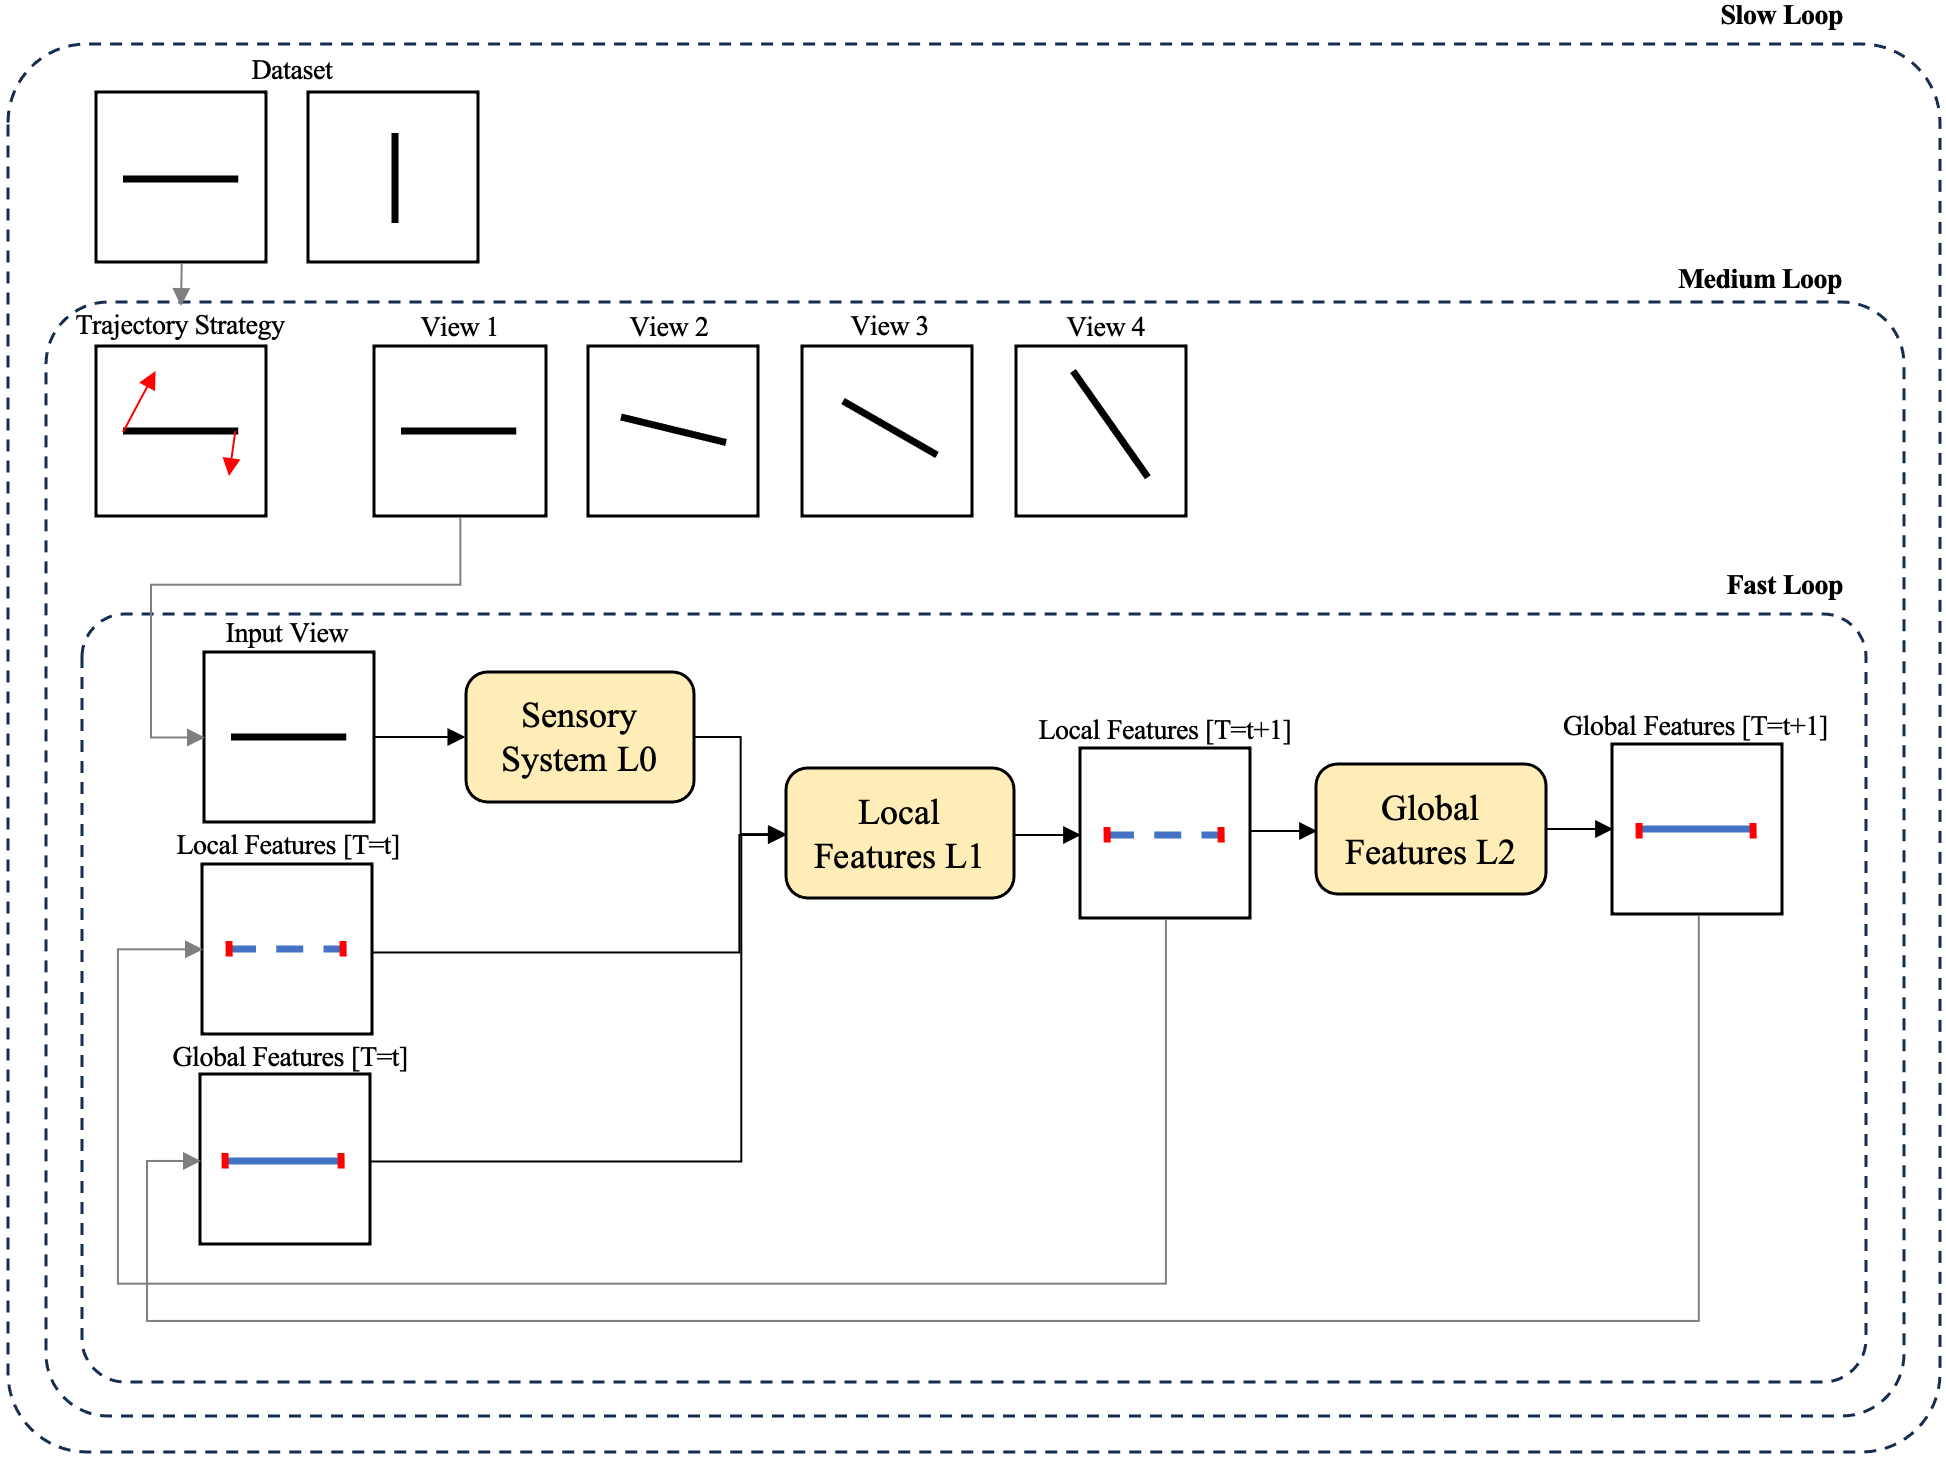
\includegraphics[width=0.99\textwidth]{lateral_loops.png}
    \caption[Processing loops of the network]{Processing loops of the network. From each sample in the dataset (slow loop), multiple views are generated (medium loop), and each view is processed over multiple timesteps by the model (fast loop).}
    \figlbl{lateral_loops}
\end{figure}

\paragraph{Slow Loop.} The dataset comprises multiple images. \figref{lateral_loops} depicts a dataset with vertical and horizontal lines, similar to the experiments conducted in this thesis (c.f. \secref{TODO}). However, depending on the application, different datasets could be used. Each image in the dataset is processed one after the other, building the outermost loop.

\paragraph{Medium Loop.} For each image in the dataset, different views are sampled using data augmentation. In the experiments conducted in this thesis (c.f. \secref{TODO}), a trajectory strategy is implemented that moves the line continuously from an initial position to a target position. This generates multiple distinct yet closely related images. Similar to our visual system, which captures multiple frames of an object before moving on to the next, this loop allows to perceive objects from various viewpoints. Furthermore, it can be used to encourage similar global features despite slight differences between the views, making the model more transformation invariant.

\paragraph{Fast Loop.} From each view, a sensory system creates neural activity that the network processes for $T$ timesteps. During these timesteps, the network iterates between building local (\emph{S1}) and global (\emph{S2}) features. The inputs in the local feature stage are the activations of the sensory system, the previous local features, and the feedback from \emph{S2} (the global features).
The activations of the sensory system can be fed into \emph{S1} only at $T=0$ or at all timesteps $T=[0, ..., t]$, whereas the previous local features and the global features are fed into \emph{S1} at $T=[1, ..., t]$. Intuitively, the goal is to iteratively improve the local features based on the previous local features and the corresponding global features. Therefore, the previous local features and the global features are required at every timestep.

The input in the global feature stage \emph{S2} are the local features extracted by \emph{S1}. The goal is to map local features to transformation invariant representations that can be used to decode a visual scene (i.e. which object is where in the image) and to provide feedback to \emph{S1}. Thus, the input data in \emph{S2} are only local features.


\section{Sensory System}
The goal of the sensory system is to perceive an input and extract multiple different features in spatially local neighbourhoods that can be used to build net fragments in the next stage.
In the case of images, the input has a shape of size $C_{\text{in}} \times W \times H$ where $C_{\text{in}}$ is the number of input channels, $W$ the image width and $H$ the image height.
The output is of shape $C_{\text{sensor}} \times W \times H$, where $C_{\text{sensor}}$ is the number of output channels. Typically, $C_{\text{sensor}}$ is much larger than $C_{\text{in}}$, i.e. $C_{\text{sensor}} \gg C_{\text{in}}$.
Each output channel represents a feature, thus the sensory system extracts at the same pixel location multiple features.

Such a sensory system to process images can be implemented by either using Gabor filters \sidecite{gabor_theory_1946, granlund_search_1978} or, in a more advanced setting, with learned filters.
Filters can be learned, for example, by training a convolutional network in an autoencoding setting \sidecite{rumelhart_learning_1986}. However, only the first layer of a convolutional network should be kept as a feature extractor to ensure that only low-level and local patterns are detected by the sensory system. The advantage of using learned filters over fixed Gabor filters is that they can be tweaked to the source data. However, this comes with the cost of additional filter training.

A difficulty is that sensory inputs are typically in continuous space and must be translated into a binary activation potential.
One option is to normalise the sensor signal in the range $0, .., 1$ and to use this value as a probability to sample from a Bernoulli distribution, similar to the proposed Bernoulli neurons (c.f. \secref{bernoulli_neuron}).
Another approach is to set all activations above a pre-defined threshold to $1$ and to assign 0 to the values below the threshold.
Alternatively, a third option is to use quantization networks such as VQ-VAEs \sidecite{van_den_oord_neural_2017} as feature extractors. Such networks can map local features to a discrete value that can be translated into a binary activation pattern.



\section{Local Feature Stage \emph{S1}}
% Subnetworks: Description and advantage
% Hebbian learning to build lateral support
% Distance of lateral connections
% Limiting lateral support with inhibition & normalization
% Alternative cells for alternative patterns
%%% Competition between graphs of lateral support structures
% Incorporating feedback from \emph{S2}
% Implementation using convolutional operations
%%%  Initialization (self-support)
%%%  Measuring support goodness

%% TODO: Gewichte erst nach letztem timestep aktualisieren

As described in \secref{model_overview}, the goal of \emph{S1} is to build local features called net fragments based on the sensory signal, the previous local features, and the global features.
Intuitively, these three types of input serve the following purposes:
\begin{itemize}
    \item \textbf{Sensory signal}: The sensory system extracts features from the image and activates cells. These initial activation are used as initial local features that are continuously sparsified by turning off cells that do not receive enough lateral support. Theoretically, the sensory signal could be used only to initialize the cell activation in \emph{S1}, However, feeding the sensory signal into the network at every timestep stabilises the activation.
    \item \textbf{Previous local features}: The local features are the output of the stage \emph{S1}. However, these features are built over multiple timesteps.
    Therefore, a recurrent connection is needed to allow access information from the previous timestep.
    \item \textbf{Global features}: The local features are mapped to object prototypes in \emph{S2} using object prototypes. An inverse function is used afterwards to map the object prototypes back to local features to provide information to \emph{S1}.
\end{itemize}

There exists various ways how these types of feedback can be combined. In this thesis, the sensory signal is stacked with the previous local features, whereby the global features can override the previous local features (c.f. \secref{TODO}).
Thus, \emph{S1} has an output shape of $C_{\text{out}} \times W \times H$ and an input shape of $C_{\text{in}} \times W \times H = C_{\text{sensor}} + C_{\text{out}} \times W \times H$.

\begin{figure}[h]
    \centering
    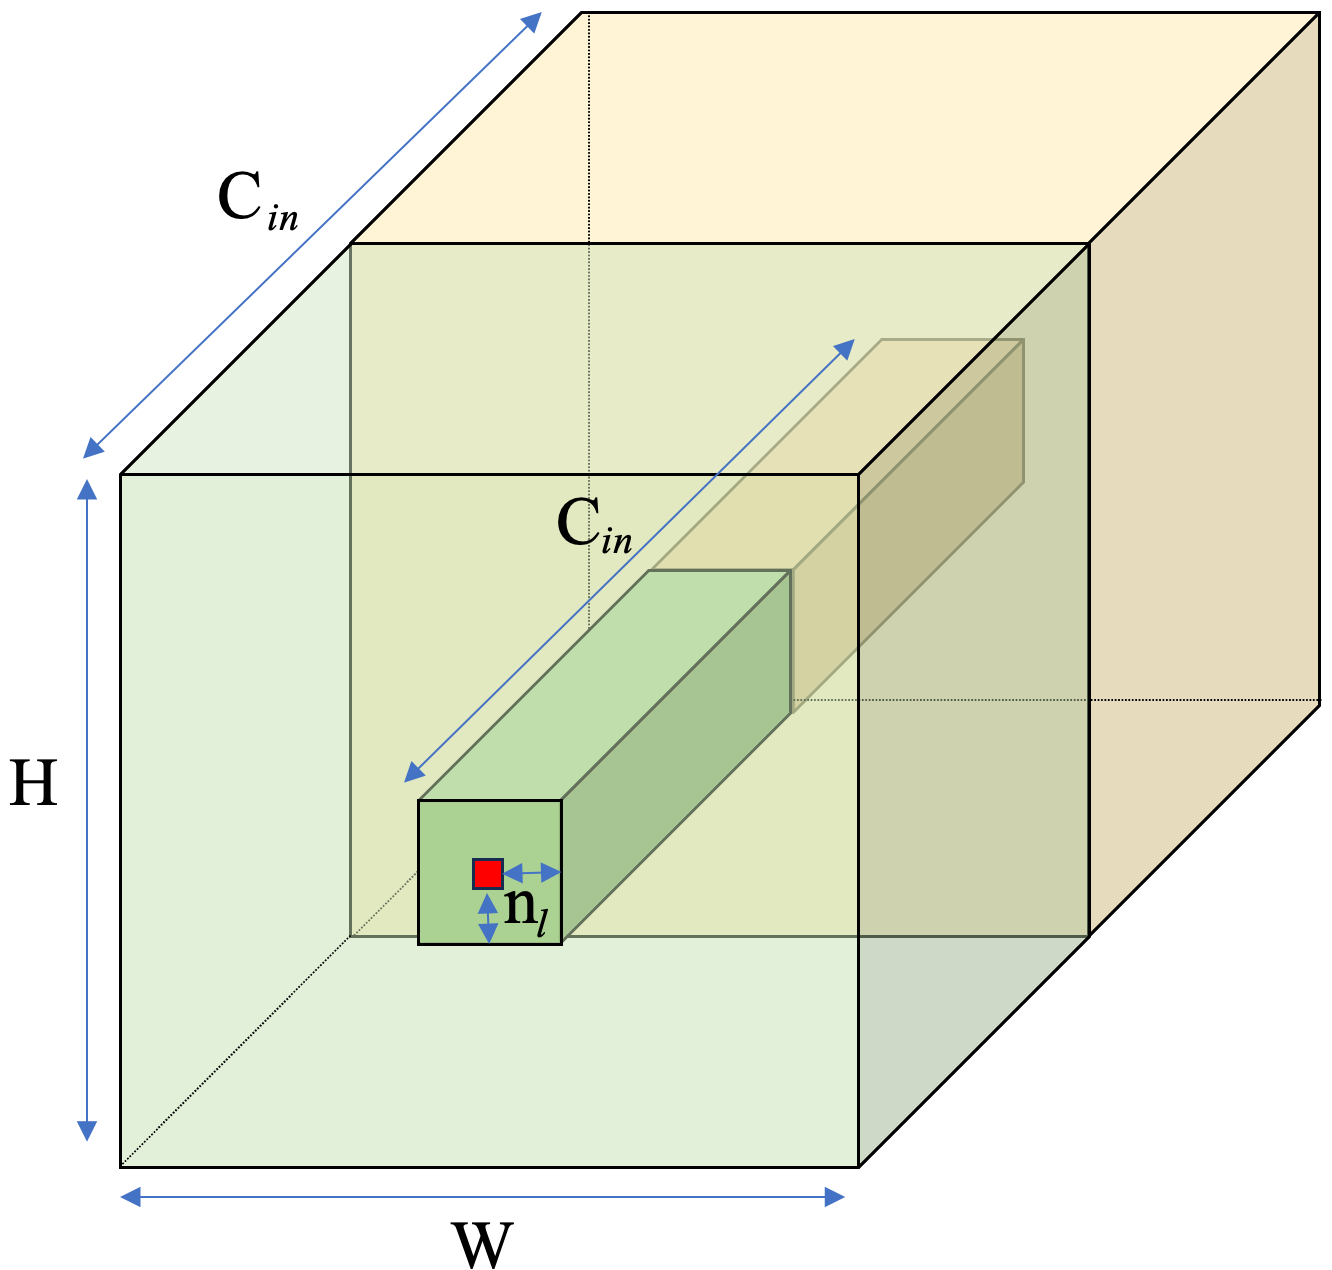
\includegraphics[width=0.99\textwidth]{local_neighbourhood.png}
    \caption[Laterally connected cells]{Visualization of the laterally connected cells: The red cell of an array of cells of the size $C_{in} \times W \times H$ is laterally connected to a neighbourhood of size  $C_{in} \times 2n \times 2n - 1$ ($-1$ representing the red cell itself).}
    \figlbl{local_neighbourhood}
\end{figure}


A single cell is denoted as $x_{c,w,h}$, where $c \in \{0, ..., C_{\text{out}}\}$ is the feature channel and $w \in \{0, ..., W\}$, $h \in \{0, ..., H\}$ the position.
These cells can initially be activated by the sensory system but are turned off by inhibitory signals rather quickly if they do not get sufficient support from spatially neighbouring cells.
The support is provided through lateral connections, i.e. connections within the same layer.
The cells are laterally connected across all input feature channels $0, ..., C_{\text{in}}$, allowing a cell to be supported by cells representing different features at the same position.
To ensure that the features in \emph{S1} remain local, the reach of the lateral connections is limited to neighbouring cells. The range of lateral connections along an image's vertical and horizontal axis is defined as $n_{l}$.
Thus, a cell $x_{c,w,h}$ has lateral connections to all cells within the range $x_{0,w-n_l,h-n_l}, ..., x_{C_{\text{in}},w+n_l,h+n_l}$.
Therefore, a single cell is laterally connected to $C_{\text{in}} \cdot 2n+1 \cdot 2n+1 = C_{\text{in}} (2n+1)^2$ neighbouring cells.
This lateral connectivity is also depicted in \figref{local_neighbourhood}. 
Please note that, according to this definition, the cell is also connected to itself.
I call this type of connection self-support.
Self-support is crucial to initialise the network properly (c.f. \secref{lateral_init}).

Patterns can appear at different locations within the image and the network should be able to recognise it independent of its spatial location \sidecite{fukushima_neocognitron_1980, waibel_phoneme_1987}. 
Therefore, lateral support should be position equivariant.
Convolutional architectures (c.f. \secref{cnns}) solve this problem with convolutional filters shifting over each pixel location. This mechanism can also be used to implement the lateral connections: When using a convolutional kernel $\boldsymbol{W}$ with size $C_{\text{out}} \times C_{\text{in}} \times 2n+1 \times 2n+1$, each output cell has a connection to its local neighbourhood as defined above.
The weights within a kernel correspond to the support strength, indicating how much a neighbouring cell supports another cell. A cell $x_{c,w,h}$ is updated as follows: 
%
\begin{align}\eqlbl{convlat_1}
	x_{c,w,h} = \sum_{c_i=0}^{C_{\text{in}}} \sum_{w_i=0}^{2n+1} \sum_{h_i=0}^{2n+1} \boldsymbol{W}_{c, c_i,w_i,h_i} \cdot x_{c_i,w-n+w_i,h-n+h_i}
\end{align}
%
Thus, the same weight $\boldsymbol{W}$ is applied at different locations and the activation strength of a cell is based on the activation strength of neighbouring cells multiplied with $\boldsymbol{W}$.


\subsection{Hebbian Updates}
The previous sections introduced how a kernel $\boldsymbol{W}$ can be used to calculate the lateral support of neighbouring cells.
In this section, it is described how the support strength, i.e. the weights of $\boldsymbol{W}$, can be learned.
The human brain's learning algorithm is based on local self-organisation and unsupervised (or self-supervised) learning \sidecite{von_der_malsburg_theory_2022}. The biologically most plausible learning algorithm is Hebbian learning \sidecite{hebb_organization_1949}. Hebbian learning can be summarized as ``neurons that fire together wire together'' (c.f. \secref{hebbian}).

The Hebbian learning rule is well suited for learning lateral connections: If two cells are active together (``fire together''), their weight increases (``wire together''). During training, the cells are activated in a specific pattern based on the sensory input. Hebbian learning strengthens the connections between the active cells, i.e., increasing the lateral support between cells that are often active together. Additionally, by using negative Hebbian learning, the strength of the lateral support can be reduced between cells that fire in disparity (one of the cells is firing while the other is not).
Thus, Hebbian learning is the algorithm to learn lateral support while being biologically plausible.

The weight $w_{ij}$ between two binary cells $x_i$ and $x_j$ is increased when they are active simultaneously. The weight update $\Delta w_{ij}$ can be calculated as follows, increasing $w_{ij}$ by the learning rate $\eta$.
\begin{align}\eqlbl{hebbu_1}
	\Delta w_{ij} = \eta x_i x_j
\end{align}
The formula above leads to an increase when both neurons are active at the same time. To decrease lateral support between cells where only one cell is active, the formula can be extended to:
\begin{align}\eqlbl{hebbu_2}
	\Delta w_{ij} = \eta \left( x_i x_j + (x_i-1) x_j + x_i (x_j -1) \right)
\end{align}
The term $(x_i-1) x_j$ becomes $-1$ if the $x_i=0$ and $x_j=1$ and thus decreases the weight if these cells are firing disparity. The second term $x_i (x_j -1)$ implements the same behaviour for the other cell ($x_i=1$ and $x_j=0$).

So far, only the update between two cells is discussed. However, the network consists of a 3D matrix of cells, each cell representing a different feature $c$ and being located at different positions $(w,h)$. In this case, a cell $x_i$ or $x_j$ corresponds to a cell $x_{c,w,h}$ within the 3D matrix of cells.

During training, the network might see similar patterns multiple times, leading to very strong connections between specific cells. The weight is normalised so that these lateral connection strengths and the post-synaptic activity cannot grow towards infinite. After calculating the weight update and adding it to the weight matrix $W$, the weights are normalised per feature channel by dividing each channel by its Euclidean norm. This ensures that the weights are roughly in the range $-1, ..., +1$.


\subsubsection{Breaking the Symmetry} 
Oja \cite{oja_simplified_1982} stated that all connections within a network trained with Hebbian learning tend to undergo the same updates and that an additional element is required to provide differentiation between the connections. Otherwise, all weights could become similar, and all feature channels depict the same features.

In practice, this additional element is typically implemented as a type of competition between the feature channels, such as a winner-take-all competition. With winner-take-all, only the neuron with the highest activation is selected for learning. In the case of our network with lateral connections, this means that at each pixel location, exactly one of the feature channels $C$ is updated. However, this is not desirable as it enforces updates even when no features are detected, leading to increased support between neurons that are not even active.

It was found that this issue can also be resolved if the probabilistic neuron is used and the network is initialised as described in \secref{lateral_init}. When using the probabilistic neuron, neurons are activated with e certain probability. Thus, neurons with a low probability tend not to fire, turning active neurons off. 
Furthermore, a proper initialisation based on self-support instead of random weights can encourages distinct feature channels.
This measures differentiation between connection updates, making a competition strategy superfluous.

\subsubsection{Implementation Details}
Implementing Hebbian updates efficiently in a deep learning framework is not trivial: In an efficient implementation, the kernel is not shifted from cell to cell. Instead, a circulant matrix is built so that all kernel updates can be calculated in parallel. However, by applying this operation, information about the cell's lateral influence is lost.

A solution to this problem is proposed by \sideciteay{miconi_hebbian_2021}. He uses a loss function whose derivative is exactly the Hebbian update. By doing so, backpropagation of error can be used to update the weights, whereby the weight update is similar to the Hebbian rule.
This allows a very efficient Hebbian training for convolutional layers.
However, this approach is quite limited and does not provide the flexibility needed to implement all parts of the proposed framework.

In this thesis, a different implementation is proposed that comes with a slight memory overhead, but is very efficient and does not rely on backpropagation at all. The proposed method is based on two convolutional layers: The first layer is a fixed, binary convolution that restructures each input patch into a single-column vector. This is followed by a $1\times1$ convolution containing the actual weights. Specifically, we can pass the input through a fixed convolution with an input size of $C_{in} \times 2n+1 \times 2n+1$ and $C_{in} 2(2n+1)$ output channels. The weight vector for this convolution is set to $1$ for the connections linking input $c_i,w,h$ to output $c_iwh$ (where $c_i$ $w$, and $h$ range from 1 to $C_{in}$, $2n+1$, and $2n+1$, respectively), and it is set to 0 everywhere else. This process reorganises the values of each input patch from the original convolution into non-overlapping column vectors, effectively duplicating them. Next, the actual weights of the original convolution using can be applied using a simple $1\times1$ convolution. This can be achieved by performing a tensor product with appropriate broadcasting.
Thus, the proposed method allows to calculate Hebbian updates while fully leveraging the computational capabilities of current deep learning hardware.














\subsubsection{Initialisation}\seclbl{lateral_init}
\begin{figure}[h]
    \centering
    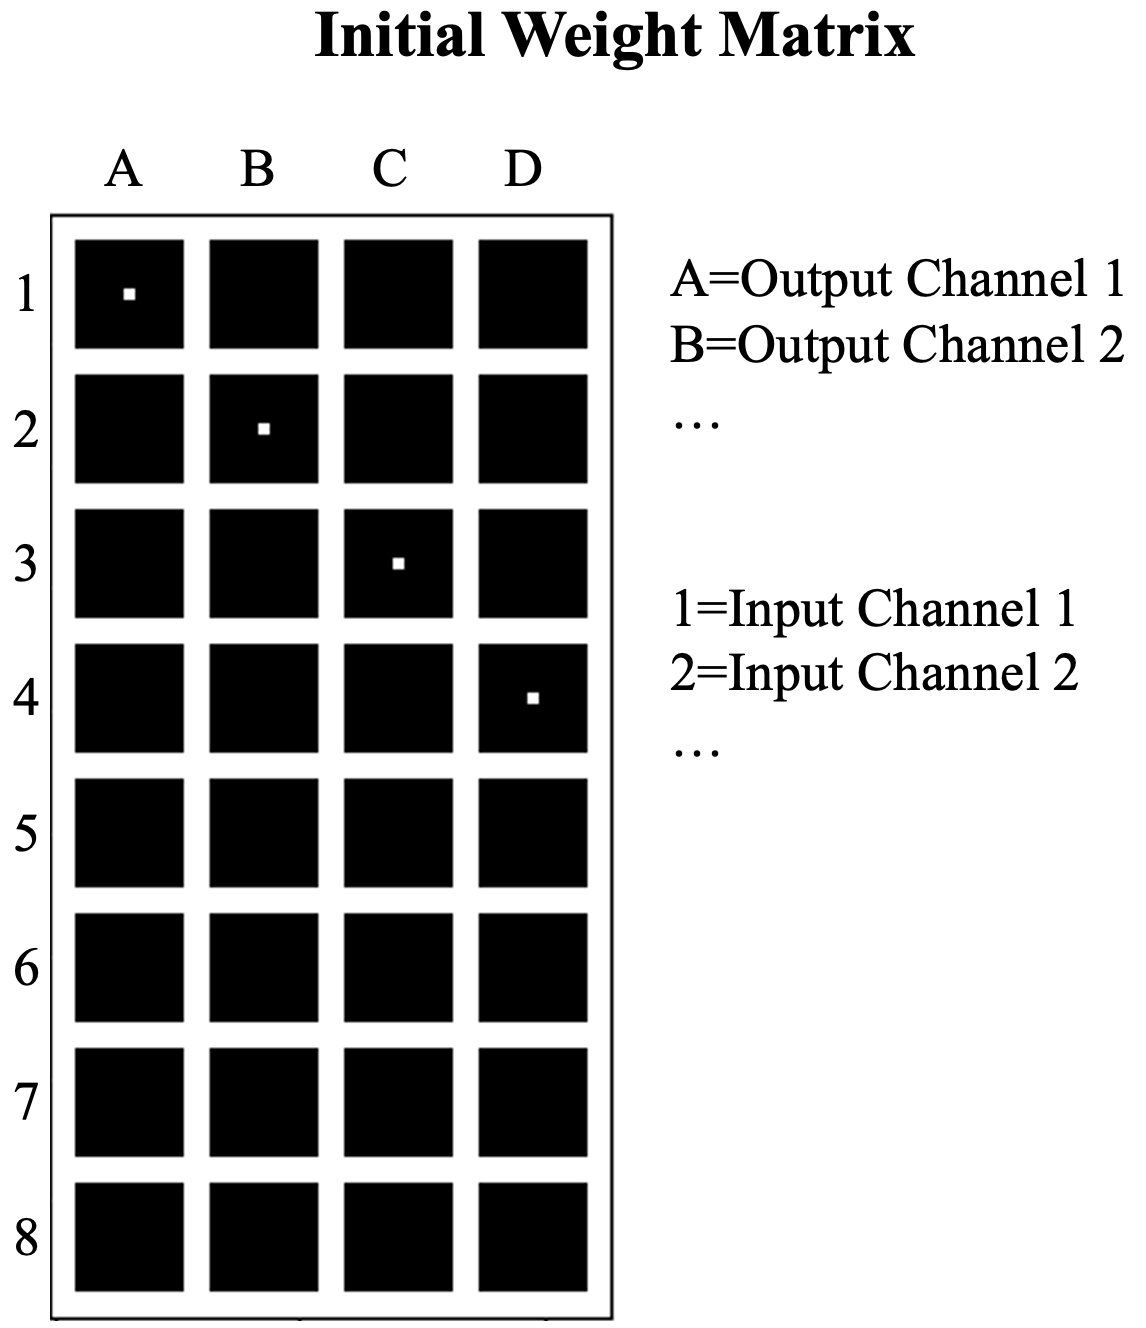
\includegraphics[width=0.6\textwidth]{lateral_init_weights.png}
    \caption[Initialization of the lateral weight matrix]{Initialization of the lateral weight matrix. The weight at the middle of a kernel, whose input and output channel have the same index, is set to $1$.}
    \figlbl{lateral_init_weights}
\end{figure}
The lateral support is implemented as weights of a convolutional kernels.
It is crucial to initialize these kernels properly, otherwise, the activations are not stable and typically converge to weights that either activate all cells or none cells.
For example, when the kernels are initialized with zeros, there is no lateral support and all cells will turn off immediately.
If the weights are initialized randomly, the initial support is random and patterns that are not in the training set  are supported.

I found that it works best if the weights are initialized with a high self-support, meaning each cell supports itself to remain active.
Self-support can be implemented by setting all weights of a kernel of size $C_{out} \times C_{in} \times w \times h$ to $1$ at the indexes that fulfil 
$C_{out} = C_{in}$, $w = n+1$, and $h = n+1$. Thus, the weight at the middle of a kernel that has the same input as output channel is set to $1$ while the other weights are set to $0$. This initialization strategy also works for kernels with a different number of input and output channels as shown in \figref{lateral_init_weights}.

Having such a weight matrix ensures that the cells activation at time $t$ and at time $t+1$ is exactly identical. However, after applying the Hebbian learning rule, the weights are updated in a way to capture the data's statistics.


\subsubsection{Normalization}
The lateral support defines the probability of a neuron to be active. However, the output of a convolutional operation is not in the range $0, ..., 1$ but can be any floating point number. Thus, this numbers have to be normalized to represent a probability.
Normalizing is quite challenging for the following reasons:
\begin{itemize}
	\item The lateral support increases over time: The lateral weights are initialized by only having self-support. However, the network's cells learn to support each other based on the data's statistics. This has the effect, that neurons become stronger activations during the course of the training process. For example, a single cell can have a binary value of $1$ at the beginning. This cell supports itself, i.e. keeps the $1$ at the beginning. After Hebbian updates, this self-support can either go towards $0$ and the cells turn off or can be supported by up to $n^2$ cells. The support strength of each of these cells can be in the range $-1, ..., 1$. Thus, a cell can have an activation up to $n^2+1$. The challenge hereby is that its initial support is $1$ and then evolves to a complete different value even if the data remains identical. Thus, the support needed to remain active must be low at the beginning of the training and be slowly increased during training until an upper bound is reached.
	\item The possible support depends on the input data: The sensory system extracts different features from the input data. Depending on the input data, there can be regions with a lot of detected features and regions with less features. For example, some areas can be constituted from many edges, and well pronounced structures leading to a lot of activations in various channels (e.g. a zebra within an image) while other areas have rather low frequencies and only a few activations (e.g. the sky in the background of the zebra image). However, even though areas have only a few activations, they should not just be turned off. Otherwise, the network would only keep features of areas with a high frequency and discard all other information.
\end{itemize}

Thus, the support depends on the learned lateral weights that change slowly during training and the input data that change every time a new scene is observed.
The problem with the changing weights can be solved by dividing the cells' activation by the sum of the lateral weights.
This normalization is done per feature channel. This allows to deal with the problem that different features receive a different strong support.
By doing so, more lateral support is needed to remain active when more lateral connections are learned: At the beginning, only self-support exists and thus the sum of the weight is $1$. Therefore, a cells activation is divided by $1$ and being active at time $t$ is enough to be active at time $t+1$.
However, during training, more lateral connections are build (i.e. more weights become $>1$). Therefore, a cells activation is divided by a value $>1$ and the activation has to be stronger to remain active with a high probability.
Mathematically, the normalization of an array of cells with an activation strength $\boldsymbol{A}(out)$ per feature channel is defined as follows:
\begin{align}\eqlbl{norm_lat}
	\boldsymbol{A}(out) :=  \boldsymbol{A}(out) / (1\cdot 10^{-10} + \sum_{ci}^{C_{in}}\sum_{w}^{2n+1}\sum_{h}^{2n+1} \boldsymbol{W(C_{out},ci,w,h)})
\end{align}

The problem that has to be solved is that the sensory system detect different features in different image areas and thus that an image's feature map depends highly on the input data. Therefore, the activations have to be normalized depending on the input data. This problem is solved by counting haw many cells are active in the lateral neighbourhood, i.e. by counting how many cells that potentially could support a cell are active.
This can be implemented efficiently by applying a convolutional operation on the input, whereby the kernel has a size of $C_{out} \times C_{in} \times 2n+1 \times 2n+1$ and all weights are set to $1$. The result of this operation is a matrix $A_{max}$, describing for each cell what its maximum activation could be for a given input.
The activations are divided element-wise by $\boldsymbol{A}_{max}$ so that they are normalized based on the sensory system's activation pattern.
\begin{align}\eqlbl{norm_lat2}
	\boldsymbol{A}(C,w,h) :=  \boldsymbol{A}(C,w,h) / \boldsymbol{A}_{max}(C,w,h)
\end{align}

The above described operations normalize the activations in a sense that they are independent from the strength of the lateral connections as well as from the input data. However, they are not bound to the range $0, ..., 1$ and, thus, not usable as probabilities.
To squeeze the activations values inside these range, min-max normalization is used.  

\begin{align}\eqlbl{norm_lat3}
	\boldsymbol{A}(C,w,h) :=  \boldsymbol{A}(C,w,h)  - \min(\boldsymbol{A}) / (\max(\boldsymbol{A}) - \min(\boldsymbol{A}))
\end{align}


\subsubsection{Measuring Support Goodness}
An open challenge from this approach is to define how good a trained network works.
A simple approach is to measure the support needed to remain active.
A simple metric is to measure the average support active and inactive cells receive.
At the beginning of training, self-support is used, i.e. it is sufficient to be active at time $t$ to remain active at $t+1$.
Therefore, the average support of active cell is $1$ and the average support of inactive cells is $0$.
However, during training, lateral connections are learned that support cells to remain active.
This leads to a higher activation in general which, in turn, increases the threshold to remain active.
Thus, the average activation of the cell increases as well as the threshold to remain active.
In a working system, the activation needed to become active increases during training.
We measure this statistics to evaluate the goodness of the subnetworks.

As a second metric, I measure the normalization factor.
The cells are activation with a specific strength based on the input and the lateral support they receive.
However, the normalization squeezes this activation into the range $0, ..., 1$.
If the cells are activated with a specific activation strength $A$ and normalized afterwards to $A_{norm}$, we can measure the normalization factor 
$\upsilon$:
\begin{align}\eqlbl{goodness_lat}
	\upsilon = \frac{A}{A_{norm}+1\cdot10^{-10}}
\end{align}
At the beginning, the cells do not receive a lot of support and thus $\upsilon$ is small. However, with increasing support, $\upsilon$ increases and indicates that a higher activation strength is needed to become active.

As a third goodness measurement, we can measure the robustness to noise.
The subnetworks consists of cells supporting each other through lateral connections. However, they should only support cells that were activated by a learned pattern. Thus, cells activated by noise should receive not receive enough support and be turned off after a few cycles.
Therefore, as a third metric, we can add noise to the input image and measure how many cells  in the sensory system are activated due to the noise and what ratio of them remains active after \emph{S1}.





\section{Global Feature Stage \emph{S2}}
% Projection fibres and \emph{S2}: Description and advantage
% Structuring of \emph{S2} -> unclear, might require some iterations to define?
% How to map \emph{S1} to \emph{S2}-> unclear, might require some iterations to define?
% Providing feedback to \emph{S1}-> unclear, might require some iterations to define?

The stage \emph{S2} combines the subnetworks of \emph{S1} to bigger and more complex structures so that entire objects can modelled, whereby an object is made up of a composition of (overlapping) subnetworks.
This mapping from subnetworks to an object representations seems to be one of the core algorithms of our visual system as it is able to solve the binding problem \sidecite{revonsuo_binding_1999, feldman_neural_2013}, i.e. answers the questions how visually perceived objects are bound together based on their properties such as shape, texture, color, contour, or motion. This process is well described in psychology and known as Gestalt phenomena \cite{ellis_source_1938, kohler_gestalt_1992, wagemans_century_2012, hamlyn_psychology_2017}, yet it is unclear how to implement it.
A promising approach seems to be to use a dynamic link architecture \sidecite{wiskott_face_1997}, 
a system of rapidly switching fibres connection netfragments from \emph{S1} and \emph{S2} based on their correlation.
However, so far, these connections were not learn with a highly flexible model such as neural network.
In this thesis, a simplified version of such projection fibres is implemented as a single linear layer\sidenote{Admittedly, this implementation is quite limited, yet still sufficient to implement a proof-of-concept of such an architecture.}.

In the proposed framework, the \emph{S2} fulfils two functions. First, it maps given subnetworks to an object representation. Therefore, local information is combined to global information, allowing us to draw conclusions about the objects within an observed scene. Second, \emph{S2} can provide feedback in the form of object probabilities to \emph{S1}, allowing \emph{S1} to update its representations over time (c.f. \secref{l2_grounding}).
Thus, \emph{S2} aims to model the conditional probabilities $P(h|x)$ of a matrix of cell activations $x$ belonging to a object prototype $h$ and vice versa $P(x|h)$.
There exist approaches that implement similar principles but suffer from a chicken-egg problem (cite work here): \emph{S1} requires feedback from \emph{S2} to build its representation while \emph{S2} requires data from \emph{S1} to build object prototypes. Therefore, most approaches typically solve this problem by hand-crafting prototypes in storing them before training in \emph{S2}. This is due to the fact that they implement projection fibres that are mapped based on the correlation between \emph{S1} and \emph{S2}, forcing representations in \emph{S1} and \emph{S2} to have a high structural similarity.
In this thesis, this problem is circumvent by using a different approach that does not require to have prototypes stored in \emph{S2} beforehand. Instead, we give \emph{S2} a certain capacity in the form of probabilistic neurons and let the network decide itself how to organize them. 
We use a linear transformation to map from $x$ to $h$ and the inverse linear transformation to map backwards from $h$ to $x$.
More specifically, we use a weight matrix $\boldsymbol{W}_{S2}$ of the size $C_{out}WH \times 16$ to map the flattened activation matrix $x$ to $h$, a binary vector of length $16$. For both mappings, we use a bias term $a$ and $b$ and calculate use the sigmoid function to squeeze the activations in the range $0, ..., 1$. 
The weight $\boldsymbol{W}_{S2}$ can be interpreted as fully connected projection fibres, mapping the cells in \emph{S1} ($x$) to cells in \emph{S2} ($h$).
\begin{align}\eqlbl{l2_1}
	P(h_j=1 | x) = \text{sigmoid}(\boldsymbol{W}_{S2} \cdot x + a) / \frac{1}{1 + e^{\boldsymbol{W}_{S2} \cdot x + a}}
\end{align}
\begin{align}\eqlbl{l2_2}
	P(x_i=1 | h) = \text{sigmoid}(\boldsymbol{W}_{S2}^\top \cdot h + b) / \frac{1}{1 + e^{\boldsymbol{W}_{S2}^\top \cdot h + b}}
\end{align}
Similar to \emph{S1}, we treat the activity of these neurons as probability and thus sample the output from a Bernoulli distribution.
\begin{align}\eqlbl{l2_3}
	h_{out} \thicksim \text{Bernoulli}(P(h | x) )
\end{align}
\begin{align}\eqlbl{l2_4}
	x_{out} \thicksim \text{Bernoulli}(P(x | h))
\end{align}

The question remaining is how to update the parameters $\boldsymbol{W}_{S2}$, $a$ ,and $b$ so that the conditional probabilities $P(h|x)$ and $P(x|h)$ are properly modelled.
Similar to a restricted Boltzman machine (RBM), we minimize the difference of the free energy function $F(\cdot)$ between $x_{in}$ and $x_{out}$ (i.e. $F(x_{in}) - F(x_{out})$) to optimize the parameters. For interested readers, I provide more details on the implementation and mathematical properties in \secref{l2_math}.

\emph{S2} thus allows to model $P(h|x)$ and $P(x|h)$, whereby $h$ is of limited size.
By minimizing the free energy function, \emph{S2} decides by itself which representation should be stored.
However, since the capacity is quite limited, \emph{S2} can only store a rather small set of representations.
When observing cell activity $x$ in \emph{S1}, $P(h|x)$ defines the probability for the cell activity in \emph{S2}. Since we sample $h_{out} \thicksim \text{Bernoulli}(P(h | x) )$, $h_{out}$ becomes binary, whereby cells with a low probability tend to be turned off, while cells with a high probability tend to fire.
This can be interpreted as filter against noise and slight deformations: A cell activity $x$ is mapped to the closest known configuration of $h$.
To provide feedback to \emph{S2}, $P(x|h)$ is calculated in a similar fashion. Thus, \emph{S2} can be interpreted as a type of probabilistic associative memory, providing feedback to \emph{S1} based on its current cell state.
However, it does not map a configuration of $x$ to a single cell (i.e. multiple cells in $h$ can be active) and thus can interpolate within the data distribution to some extend.

One problem is that at the beginning of training, \emph{S1} and \emph{S2} are rather unstructured and their cell activation may change rather strongly.
For example, the feedback from \emph{S2} evolves from initial noise and is, therefore, not only useless for \emph{S1} but harmful as it can provide wrong feedback and steer learning process of \emph{S1} towards a wrong direction (i.e. \emph{S1} learns to build noise instead of proper subnetworks).
Therefore, the feedback of \emph{S2} to \emph{S1} is turned off during the first training epochs.
This allows \emph{S1} to learn subnetworks and to forward its activation to \emph{S2}. \emph{S2}, on the other hand, organizes its internal structure which takes a few epochs.
After \emph{S2} is well organized and its feedback is helpful for \emph{S1}, the feedback loop is activated.



\subsubsection{Mathematical Details}\seclbl{l2_math}
To model the conditional probability between $x$ and $h$, we have to measure their compatibility (i.e. to measure their relationship).
Lets imagine two cells $x_i$ and $h_j$ and the weight $\boldsymbol{W}_{ij}$ to model the connection between these cells.
Intuitively, $\boldsymbol{W}_{ij}$ indicates whether $x_i$ and $x_j$ are positively or negatively related: If $x_i$ and $h_j$ are equal, we want $\boldsymbol{W}_{ij} > 0$ and $\boldsymbol{W}_{ij} < 0$ otherwise.
The energy function $E(x_i, h_j)$ is defined as
\begin{align}\eqlbl{l2_energy}
	E(x_i, h_j) = - \boldsymbol{W}_{ij}x_ih_j
\end{align}
The energy function is high, if $x_i=h_j=1$ and the weight is wrong, i.e. $\boldsymbol{W}_{ij} < 0$. The energy function with the biases can be formulated as
\begin{align}\eqlbl{l2_energy2}
	E(x_i, h_j) = - \boldsymbol{W}_{ij}x_ih_j - a_ix_i - b_jh_j
\end{align}
The energy function for the entire network is the sum of all units:
\begin{align}\eqlbl{l2_energy3}
	E(x, h) = - \sum_{i,j} \boldsymbol{W}_{ij}x_ih_j - \sum_ia_ix_i - \sum_jb_jh_j
\end{align}
To probability for a pair of \emph{S1} cell activations $x$ and \emph{S2} cell activations $h$ can be calculated as:
\begin{align}\eqlbl{l2_energy4}
	P(x,h) = \frac{e^{-E(x, h)}}{Z}
\end{align}
where the partition function $Z$ is the sum from all possible states and can be calculated as:
\begin{align}\eqlbl{l2_energy5}
	Z = \sum_{x,h} = e^{-E(x,h)}
\end{align}
The probability for a cell state in \emph{S1} can be calculated by summing over all cell states of \emph{S2}:
\begin{align}\eqlbl{l2_energy6}
	P(x) = \frac{1}{Z} \sum_{h}e^{-E(x,h)}
\end{align}
This probability $P(x)$ of observing state $x$ in \emph{S1} can be used to learn the weights. In fact, the probability that the models assigns to a specific cell state can be raised by lower the energy of that cell state and to raise the energy of other cell states. I.e. the weights are adapted in a way that this cell state becomes more probable while other cell states become less probable.
To update the weights, we have to calculate the derivative of the log probability of a cell state $x$ w.r.t. the parameters $\theta$:
\begin{align}\eqlbl{l2_energy7}
	\frac{\partial \log P(x)}{\partial \theta }
\end{align}
This derivative can be calculated with the free energy function. The free energy of a cell state $x$ describes the ``available energy'' and is the sum of all energy configurations that contain $x$.
\begin{align}\eqlbl{l2_energy8}
	F(x) = \ln \left( \sum_h e^{-E(x,h)} \right)
\end{align}
Without any proof, the derivative of the log probability of a cell state $x$ w.r.t. the parameters $\theta$ can be calculated as follows:
\begin{align}\eqlbl{l2_energy9}
	\frac{\partial \log P(x)}{\partial \theta } = - \frac{\partial \mathcal{F}(x)}{\partial \theta} + \mathbb{E}_{x' \sim p} \left[ \frac{\partial \mathcal{F}(x')}{\partial \theta}  \right]
\end{align}

Thereby, $x$ is the original cell state of \emph{S1} and $x'$ a reconstructed version of it.
The reconstructed version $x'$ can be calculated by mapping $x$ to an object prototype in \emph{S2}  $h \thicksim \text{Bernoulli}(P(h | x) )$ and sampling from $h$, i.e. $x' \thicksim \text{Bernoulli}(P(x | h))$.
Thus, the loss can be calculated by minimizing $F(x) - F(x')$ w.r.t. $\theta$ by using gradient descent.


% https://jhui.github.io/2017/01/15/Machine-learning-Boltzmann-machines/#:~:text=The%20free%20energy%20of%20RBM,(1%2Bexj)


%\subsubsection{Self-Consistency and Parsimony}
%A fundamental task of all learning frameworks is to define how data should be organized.
%Studies in neuroscience suggest that the brain’s world model is highly structured \sidecite{Olshausen_Field_1996, Bao_She_McGill_Tsao_2020}.
%The key to the brain's efficiency and effectiveness in perceiving, predicting, and making intelligent decisions is thought to lie in a structured model \sidecite{Josselyn_Tonegawa_2020}.
%Some of the most important principles of such a structured model is parsimony and self-consistency \sidecite{Ma_Tsao_Shum_2022}.
%In this thesis, the world model is encoded in \emph{S2}.
%\emph{S2} learns object prototypes that are arranged in its feature space in a self-organizing manner.
%However, constraints inspired by the principles of parsimony and self-consistency ensure that these features are organized in a meaningful way.

%The principle of parsimony is to identify low-dimensional structures in the data and to reorganize them in the most compact and structured way.
%According \cite{Ma_Tsao_Shum_2022}, this can be achieved with compression, linearization, and sparsification.
%Compression is achieved by mapping the cell's activity in \emph{S1} to a low-dimensional representation in \emph{S2}. In fact, we reduce a martix of size $4\times32\times32$ to a vector of size $1\times16$, thus compressing the data by a factor of $256$.
%\emph{S2} uses binary neurons, whereby each neuron represents a specific feature.
%Since the activations in \emph{S1} depend strongly on the data (i.e. are low-level features), they vary a lot.
%\emph{S2}, on the other hand, tries to capture the this diversity as good as possible by minimizing its weights' free energy.
%Therefore, each neuron in \emph{S2} represents a quite unique feature, leading to sparse representations (TODO reference sparse coding).
%However, I do not enforce a orthogonal features (a ``one-hot'' encoding). This is also in line with the human brain where more than one cell is active in specific brain regions (cite).
%But the aforementioned constraints lead to such sparse cell activations in \emph{S2}, that only a few (on average $4$ out of $16$) cells are active.
%Thus, \emph{S2} encourages linearization while fulfilling compression and sparsification. Therefore, I argue that it implements the principle of parsimony to a large extend.

%The principle of self-consistency describes that a network should seek the most self-consistent world-model by minimizing the internal discrepancy between representations of observed and regenerated data.
%\emph{S2} is trained to minimize the free energy of $x$ and $\hat{x}$, thus optimizing the free energy of the weights w.r.t. the outer representations. However,  \emph{S2} is not implemented with a separate encoder and decoder. Instead, the mapping of the encoder is based on a linear weight matrix $\boldsymbol{W}$, and the decoder is based on the transposed weight matrix $\boldsymbol{W}^\top$. 


%TODO: Self-Consistency -> Why??


\subsubsection{Measuring \emph{S2} Goodness}
\emph{S2} maps activations of learned patterns to object prototypes and vice-versa.
It can be interpreted as a type of associative memory with the capability of interpolating within the data distribution.
Thereby, it should be more robust to noise and slight image transformation than \emph{S1}.
Thus, the goodness of \emph{S2} can be measured in terms of reconstruction of transformed or partially masked objects and removing noise.


- Reconstruct Lines
- Remove noise (not removed by \emph{S1})



\subsection{Limitations}
The proposed framework is an interesting alternative to current vision architectures.
However, it still has many drawbacks and requires further research to improve certain aspects.
The most pressing issues, from the author's perspective, are described in the following.

The core idea is to build subnetworks in \emph{S1} and to map them to 


- How to put prototypes into \emph{S2}
- Multi-step projection fibres based on correlation
- position invariance \emph{S2}
- unbalanced data (i.e. some patterns dominate \emph{S1}) -> probabilistic neuron is not enough -> requires competition to learn
- Mehrere parallele identische Zellen nötig, damit sich verschiedene Feature-Kombinationen ausbilden können (z.B. Feature 1+2 ohne 3 aber auch Feature 1+3)


TODO
- Neue Normalisierung beschreiben
- Hemmung beschreiben
- Beschreiben, dass alternative Zellen nötig sind für verschiedene Muster -> Symmetrieproblem -> Benötigt eine Art Competition -> Evtl. können sich Zellen bei zu viel Aktivität sogar selbstständig verdoppeln




TODO: teste was passiert wenn Noise in Feature Extractor statt Image -> wird dieser entfernt?
TODO: Teste anderen Noise, z.B. Kreis


TODO \emph{S2}: https://devpost.com/software/recursive-cortical-network-visualizations

TODO: Chaining multiple \emph{S1} - \emph{S2} stages. Could a stage serve as \emph{S1} and \emph{S2} at the same time? -> Build a chain of stage?